\documentclass[11pt, a4paper]{article}
\usepackage[a4paper, margin=2.5cm]{geometry}\usepackage[T1, T5]{fontenc}
\usepackage[utf8]{inputenc}
\usepackage{mathptmx} % Cung cấp font giống hệt Times New Roman
\usepackage[english]{babel}
\usepackage{booktabs}
\usepackage{array}
\usepackage{float}
\usepackage{graphicx}
\usepackage{hyperref}

\title{EARTH SCIENCE FIELDTRIP REPORT}
\author{Group 83}
\date{May 2026}

\begin{document}

% --- TITLE PAGE ---
\begin{titlepage}
    \centering
    \vspace*{1cm}
    
    {\large \textbf{VIETNAM NATIONAL UNIVERSITY HO CHI MINH CITY} \\
    \textbf{HO CHI MINH CITY UNIVERSITY OF TECHNOLOGY} \\
    \textbf{FACULTY OF GEOLOGY AND PETROLEUM ENGINEERING} \par}
    
    \vspace{4cm}
    
    {\Large Earth Science \par}
    \vspace{0.5cm}
    {\Huge \textbf{EARTH SCIENCE FIELDTRIP REPORT} \par}
    
    \vspace{3cm}
    
    \begin{table}[h]
        \centering
        \large
        \renewcommand{\arraystretch}{1.5}
        \begin{tabular}{>{\bfseries}l l}
            Advisor: & Dr. Nguyễn Ngọc Thủy \\
            Class: & A02 \\
            Group: & 35 \\
            Students: & Hồ Công Thành - 2313111 \\
                      & Nguyễn Đình Huy -  \\
                      & Nguyễn Thành Nhân -  \\
                      & Thái Khắc Hùng -  \\
                      & Phan Nguyễn Khánh Mai - 2211988 \\
        \end{tabular}
    \end{table}
    
    \vfill
    
    {\large HO CHI MINH CITY, May 2026 \par}
\end{titlepage}

% --- TABLE OF CONTENTS ---
\tableofcontents
\newpage
\listoffigures
\listoftables
\newpage

% --- MAIN DOCUMENT ---
\section{Introduction}

\subsection{Purpose of Preparing the Field Trip Report}
The purpose of this field trip report is to summarize, organize, and interpret the observations collected during the Earth Science fieldtrip. Instead of describing the visited locations only in the order of the itinerary, this report follows the structure of Earth systems, including the geosphere, hydrosphere, biosphere, atmosphere, and natural resources.

Through the fieldtrip, students had the opportunity to observe geological materials and natural processes directly in real environments. The report focuses on connecting field evidence with theoretical knowledge learned in class, such as rock formation, weathering, sediment transportation, coastal processes, groundwater, and the use of geological resources in human activities.

Preparing this report also helped students develop important academic and fieldwork skills. These include taking field notes, collecting rock and sediment samples, using maps and compasses, taking photographs, recording videos, and interpreting geological features based on real observations. Therefore, the report serves not only as a summary of the fieldtrip but also as a reflection of the learning process and teamwork during the course.

\subsection{Task Assignment Table of Group Members}
During the fieldtrip, each member was assigned specific responsibilities to make sure that observations were recorded systematically and samples were collected properly. Although each student had a main task, all members supported one another during observation, discussion, sample collection, and documentation.

\begin{table}[htbp]
    \centering
    \caption{Task assignment of group members}
    \begin{tabular}{clp{9cm}}
        \toprule
        \textbf{No.} & \textbf{Name} & \textbf{Main Tasks} \\
        \midrule
        1 & Nguyễn Trung Nhân & Following the lecturer closely and collecting rock samples. \\
        2 & Nguyễn Vĩnh Phú & Collecting samples and extracting sample information for observation. \\
        3 & Nguyễn Kim Hoàng Phi & Collecting samples during field observations. \\
        4 & Phan Nguyễn Khánh Mai & Taking notes and taking photos during the fieldtrip. \\
        5 & Nguyễn Thị Yến Nhi & Taking notes and recording videos during the fieldtrip. \\
        \bottomrule
    \end{tabular}
\end{table}

\subsection{Natural, Technical, and Socio-economic Characteristics of the Study Area}
The fieldtrip was conducted in Vung Tau and nearby areas, where students could observe a combination of natural landscapes, geological outcrops, coastal environments, and industrial facilities. The study area includes old and active quarries, coastal beaches, sand dune systems, hillside terrain, and petroleum-related industrial sites. These locations provided suitable conditions for studying Earth Science concepts in real field settings.

From a natural perspective, the study area contains diverse geological materials and landforms. At VNU Lake, students observed andesite, an extrusive igneous rock related to volcanic activity. At Gia Quy Quarry, basaltic materials, pozzolan, and spheroidal weathering features were observed. At Sao Mai Quarry, granite and diabase provided evidence of intrusive igneous activity and cross-cutting relationships. Coastal locations such as Back Beach and Cua Lap showed marine sediments, aeolian sand dunes, coastal transportation, and deposition processes. The Lighthouse area provided a broader view of hillside terrain and coastal geomorphology.

From a technical perspective, the fieldtrip helped students practice basic geological field methods. These included collecting rock and sediment samples, using maps and compasses, recording field notes, taking photographs, and observing rock structures and sedimentary features. The use of smartphones and the Clino app also supported basic field measurements and documentation.

From a socio-economic perspective, the study area demonstrates the relationship between geology and human activities. Gia Quy Quarry shows the extraction and use of basaltic and pozzolanic materials for construction and cement-related applications. Vietsovpetro represents the petroleum service industry in Vung Tau and shows how geological knowledge is applied in offshore exploration, energy production, and industrial development. Therefore, the fieldtrip area is valuable not only for geological study but also for understanding the practical role of Earth Science in society.

\subsection{Tentative Schedule}
The Earth Science fieldtrip was organized over three days in Vung Tau and nearby coastal areas. Before the departure, a general fieldtrip plan was prepared to ensure that all activities, observation sites, and learning objectives could be completed effectively. The schedule included geological observations at igneous rock outcrops, coastal sedimentary environments, mining areas, and industrial locations related to petroleum geology.

The fieldtrip was designed to help students connect theoretical geological knowledge with practical field observations. At each location, students conducted geological observations, identified rock and sediment characteristics, analyzed geological structures, and discussed geological processes under the guidance of the lecturers.

\subsubsection{General Planning Schedule}
The following figure presents the official fieldtrip schedule prepared before the excursion.

\begin{figure}[htbp]
    \centering
    [Image: Official fieldtrip schedule for Earth Science (GE1013)]
    \caption{Official fieldtrip schedule for Earth Science (GE1013).}
\end{figure}

The planned schedule included several important observation sites such as VNU Lake, Gia Quy Quarry, Sao Mai Quarry, Back Beach, Cua Lap, Vietsovpetro, and the Lighthouse area. Each site focused on different geological topics including igneous rocks, weathering, sedimentary processes, coastal geology, structural relationships, and industrial applications of geology.

\subsubsection{Actual Fieldtrip Activities}
During the fieldtrip, students participated in geological observations and practical activities at each scheduled stop. The activities included rock identification, sediment observation, structural interpretation, sample collection, field documentation, and discussions with lecturers regarding geological processes and environmental conditions.

\begin{table}[htbp]
    \centering
    \caption{Overview of actual fieldtrip activities and geological topics}
    \begin{tabular}{p{2cm} p{2cm} p{3.5cm} p{4.5cm} p{2.5cm}}
        \toprule
        \textbf{Date/Time} & \textbf{Location} & \textbf{Coordinates} & \textbf{Main Activities} & \textbf{Main Topics} \\
        \midrule
        7:00 AM \newline May 8, 2026 & Ho Da VNU & Latitude: 10.877268°N \newline Longitude: 106.790556°E & Observing andesite, describing rock characteristics, and practicing field observation techniques. & Andesite; laterite \\
        \midrule
        11:00 AM \newline May 8, 2026 & Gia Quy Quarry & Latitude: 10.503907°N \newline Longitude: 107.272151°E & Identifying basalt, observing volcanic textures, weathering features, and the mining environment. & Basalt; weathering; mining \\
        \midrule
        2:30 PM \newline May 8, 2026 & Sao Mai Quarry & Latitude: 10.385507°N \newline Longitude: 107.063481°E & Observing granite and diabase, studying cross-cutting relationships, and collecting rock samples. & Granite; diabase; intrusion \\
        \midrule
        5:30 PM \newline May 8, 2026 & Back Beach & Latitude: 10.328259°N \newline Longitude: 107.088303°E & Observing marine sediments, analyzing beach sand, and studying coastal transportation and deposition. & Marine sediments; coastal processes \\
        \midrule
        7:00 AM \newline May 9, 2026 & Cua Lap & Latitude: 10.390890°N \newline Longitude: 107.158205°E & Studying coastal sediments, Aeolian sand dunes, groundwater conditions, and sedimentary processes. & Aeolian sediments; groundwater \\
        \midrule
        9:30 AM \newline May 9, 2026 & Vietsovpetro & Latitude: 10.360200°N \newline Longitude: 107.084696°E & Attending an industry visit, learning about petroleum-related applications of geology, and joining an orientation session. & Petroleum industry; energy resources \\
        \midrule
        7:00 AM \newline May 10, 2026 & Lighthouse & Latitude: 10.334079°N \newline Longitude: 107.077631°E & Observing coastal landscapes, hillside terrain, and panoramic views of Vung Tau City and the surrounding sea during the Lighthouse observation activity. & Coastal geomorphology; landscape \\
        \bottomrule
    \end{tabular}
\end{table}

Overall, the fieldtrip activities were completed successfully and provided students with valuable practical experience in geological observation and interpretation. The combination of field investigation, group discussion, and direct interaction with geological features helped strengthen students' understanding of Earth Science concepts learned in class.

\section{Geosphere}

\subsection{Weathering in Laterite and Formation Mechanism}
Laterite is a weathering product commonly formed in tropical regions where the climate is hot and humid. Under these conditions, rainwater infiltrates into the ground and causes strong chemical weathering of the original parent rock. During this process, soluble elements such as silica, calcium, sodium, and potassium are gradually leached away, while less soluble iron and aluminum compounds remain and become concentrated.

The reddish-brown to yellowish color of laterite is mainly caused by the enrichment of iron oxides and hydroxides. These minerals form when iron-bearing minerals in the parent rock react with oxygen and water. As weathering continues, the material becomes harder and more compact, producing a rough and nodular surface. This explains why laterite often appears as a reddish, porous, and strongly weathered rock-like material.

In this fieldtrip, laterite was observed as a weathered material with brown, yellow, and reddish tones. The sample showed a rough surface with many small particles and iron-rich patches, indicating long-term chemical weathering under tropical environmental conditions.

\begin{figure}[htbp]
    \centering
    [Image: Laterite sample]
    \caption{Laterite sample showing reddish-brown color and rough weathered texture.}
\end{figure}

The observation of laterite helped students understand that weathering is not only a process of breaking rocks into smaller pieces, but also a chemical transformation of minerals. In this case, the strong leaching process removed mobile elements and left behind iron-rich materials, forming laterite.

\subsection{Erosion and Coastal Processes}
Coastal erosion is the process in which waves, currents, tides, and wind remove and transport sediments or rock materials from the shoreline. In coastal environments, erosion and deposition often occur together. While some areas lose sediments due to wave attack, other areas receive and accumulate transported materials.

At Cua Lap, students observed sandy surfaces shaped by wind and coastal processes. The sand surface showed ripple-like patterns, which are small sedimentary structures formed by the movement of wind over loose sand. These features indicate that wind is an important transportation agent in this area. Dry sand particles are moved across the surface and gradually accumulate to form aeolian sand deposits.

\begin{figure}[htbp]
    \centering
    [Image: Wind-shaped sand surface]
    \caption{Wind-shaped sand surface and ripple-like structures observed at Cua Lap.}
\end{figure}

The observation at Cua Lap demonstrates the interaction between the atmosphere, hydrosphere, and geosphere. Wind transports dry sand inland, while waves and coastal currents continuously rework beach sediments near the shoreline. As a result, the coastal area is constantly modified by erosion, transportation, and deposition.

These processes are important because they control the shape of beaches, sand dunes, and coastal landforms. They also influence coastal stability and may affect human activities in nearby areas.

\subsection{Magma Eruption Processes and Rhyolite}
Rhyolite is an extrusive igneous rock formed from silica-rich lava. It is produced when magma erupts onto or near the Earth's surface and cools rapidly. Because rhyolitic magma contains a high amount of silica, it is usually more viscous than basaltic magma. As a result, rhyolite is commonly associated with volcanic activity, lava domes, and sometimes explosive eruptions.

During the fieldtrip, rhyolite was observed in the coastal area of Vung Tau. The rock surfaces showed dark grey, purplish, reddish-brown, and weathered colors. These color variations may be related to mineral composition, oxidation of iron-bearing minerals, and long-term exposure to coastal weathering conditions. The observed rhyolite also showed fractures and irregular rock blocks, indicating that the rock had been affected by both volcanic formation processes and later surface weathering.

\begin{figure}[htbp]
    \centering
    [Image: Rhyolite surface]
    \caption{Rhyolite surface observed near the coastal area of Vung Tau.}
\end{figure}

The rhyolite outcrop near the coast provided a clear example of volcanic rock exposed at the Earth's surface. Since rhyolite forms from erupted lava, it represents past magma eruption processes in the geological history of the area. Compared with basalt, rhyolite is generally richer in silica and may display lighter, reddish, or purplish tones depending on oxidation and alteration.

In addition, the coastal setting influenced the appearance of the rhyolite outcrop. Sea waves, saltwater, wind, rainfall, and temperature changes can gradually weather exposed rock surfaces and widen existing cracks. Therefore, the site shows how an igneous rock formed by endogenous processes can later be modified by exogenous processes such as weathering and coastal erosion.

\begin{figure}[htbp]
    \centering
    [Image: Fractured and weathered rhyolite]
    \caption{Fractured and weathered rhyolite outcrop near the coastal area of Vung Tau.}
\end{figure}

The observation helped students understand that rhyolite is not only evidence of past volcanic activity, but also a rock type that continues to be changed after formation. The fractures, weathered surfaces, and coastal exposure demonstrate the combined effects of magma eruption, structural cracking, oxidation, and coastal weathering.

\subsection{Granitic Intrusion, Diabase Dykes, and Cross-cutting Relationships}

\subsubsection{Granitic Intrusion}
Granite is an intrusive igneous rock formed when magma cools slowly beneath the Earth's surface. Because the cooling process happens underground and takes a long time, mineral crystals have enough time to grow. Therefore, granite usually has a coarse-grained texture, with visible mineral grains such as quartz and feldspar.

At Sao Mai Quarry, granite appeared as a light-colored rock body with a coarse crystalline texture. The rock was mainly whitish to light grey, with visible dark and light mineral grains. This observation indicates that the granite formed through slow crystallization of magma below the surface before being exposed by later uplift, erosion, or quarrying activities.

\begin{figure}[htbp]
    \centering
    [Image: Light-colored granite]
    \caption{Light-colored granite observed at Sao Mai Quarry.}
\end{figure}

\subsubsection{Diabase Dykes}
Diabase is another intrusive igneous rock observed during the fieldtrip. Unlike granite, diabase is darker in color and usually has a finer texture. It commonly occurs as a dyke, which forms when magma intrudes into cracks or fractures of pre-existing rocks and then solidifies.

At Sao Mai Quarry, diabase appeared as a dark grey to greenish-grey rock. Its darker color and finer texture made it clearly different from the surrounding granite. The presence of diabase indicates that after the granite had already formed, new magma later intruded into fractures inside the older rock body.

\begin{figure}[htbp]
    \centering
    [Image: Dark-colored diabase]
    \caption{Dark-colored diabase observed at Sao Mai Quarry.}
\end{figure}

\subsubsection{Cross-cutting Relationship of Intrusive Igneous Rocks}
One of the most important geological features observed at Sao Mai Quarry was the cross-cutting relationship between diabase and granite. In the outcrop, the darker diabase body was seen cutting across the lighter granite body. This relationship is important because it helps determine the relative age of the rocks.

According to the principle of cross-cutting relationships, a geological body that cuts through another rock must be younger than the rock it cuts. Therefore, the diabase dyke is younger than the granite. This means that the granite formed first, and later, diabase magma intruded into fractures within the granite and solidified.

\begin{figure}[htbp]
    \centering
    [Image: Diabase cutting granite]
    \caption{Dark diabase cutting through light-colored granite at Sao Mai Quarry.}
\end{figure}

This field evidence helped students understand how geologists reconstruct the sequence of geological events. Instead of only identifying rock types, students could interpret which rock formed earlier and which formed later based on their relationships in the field.

\subsection{Summary of Geosphere Observations}
The geosphere observations during the fieldtrip showed several important geological processes. Laterite represented intense chemical weathering under tropical conditions. Cua Lap illustrated coastal erosion, wind transportation, and sand deposition. Rhyolite demonstrated volcanic eruption processes and the formation of extrusive igneous rocks. Sao Mai Quarry showed intrusive igneous activity through granite and diabase, especially the cross-cutting relationship between the two rock types.

Overall, these observations helped students understand how rocks are formed, modified, weathered, and exposed at the Earth's surface. They also showed that geological features in the field can be used to interpret the formation history and relative timing of geological events.


\section{Hydrosphere}

\subsection{Surface Water and Stream Processes at Suoi Tien (Fairy Stream)}
Suoi Tien (Fairy Stream) represents a unique surface water system flowing through a micro-canyon terrain shaped by wind and water erosion. The shallow stream is characterized by a steady, low-velocity laminar-to-turbulent flow that constantly transports fine sand particles down to coastal estuaries.

As surface water flows along the channel, it continuously undercuts the base of the surrounding sand and clay cliffs. This lateral stream erosion, combined with rainfall runoff, causes small-scale slope instability and mass wasting along the stream margins. The interaction between surface water and weathered sand formations demonstrates active fluvial-aeolian erosion and sediment transport within a coastal stream environment.

\begin{figure}[H]
    \centering
    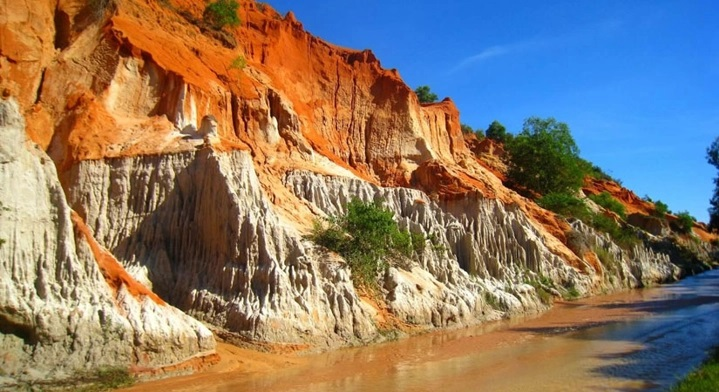
\includegraphics[width=0.8\textwidth]{images/suoi_tien.jpg}
    \caption{Surface water flow and undercut sand cliffs observed at Suoi Tien.}
    \label{fig:suoi_tien}
\end{figure}

\subsection{Groundwater Dynamics in Coastal Sand Dune Systems (Ho Tram \& Coastal Dunes)}
Coastal sand dunes, such as those observed around Ho Tram and adjacent coastal stretches, play a critical role in local hydrogeology. Because loose dune sand possesses high porosity and permeability, rainwater easily infiltrates directly into the subsurface with minimal surface runoff, establishing these dune fields as effective natural groundwater recharge zones.

Rainwater penetrating through the sandy layers forms a shallow freshwater lens above denser saline water. During field observations, local groundwater wells and natural seepages along dune depressions demonstrated the availability of accessible freshwater in sandy environments. However, these shallow aquifers remain highly sensitive to over-extraction and sea-level fluctuations, which can trigger saltwater intrusion into the fresh groundwater zone.

\begin{figure}[htbp]
    \centering
    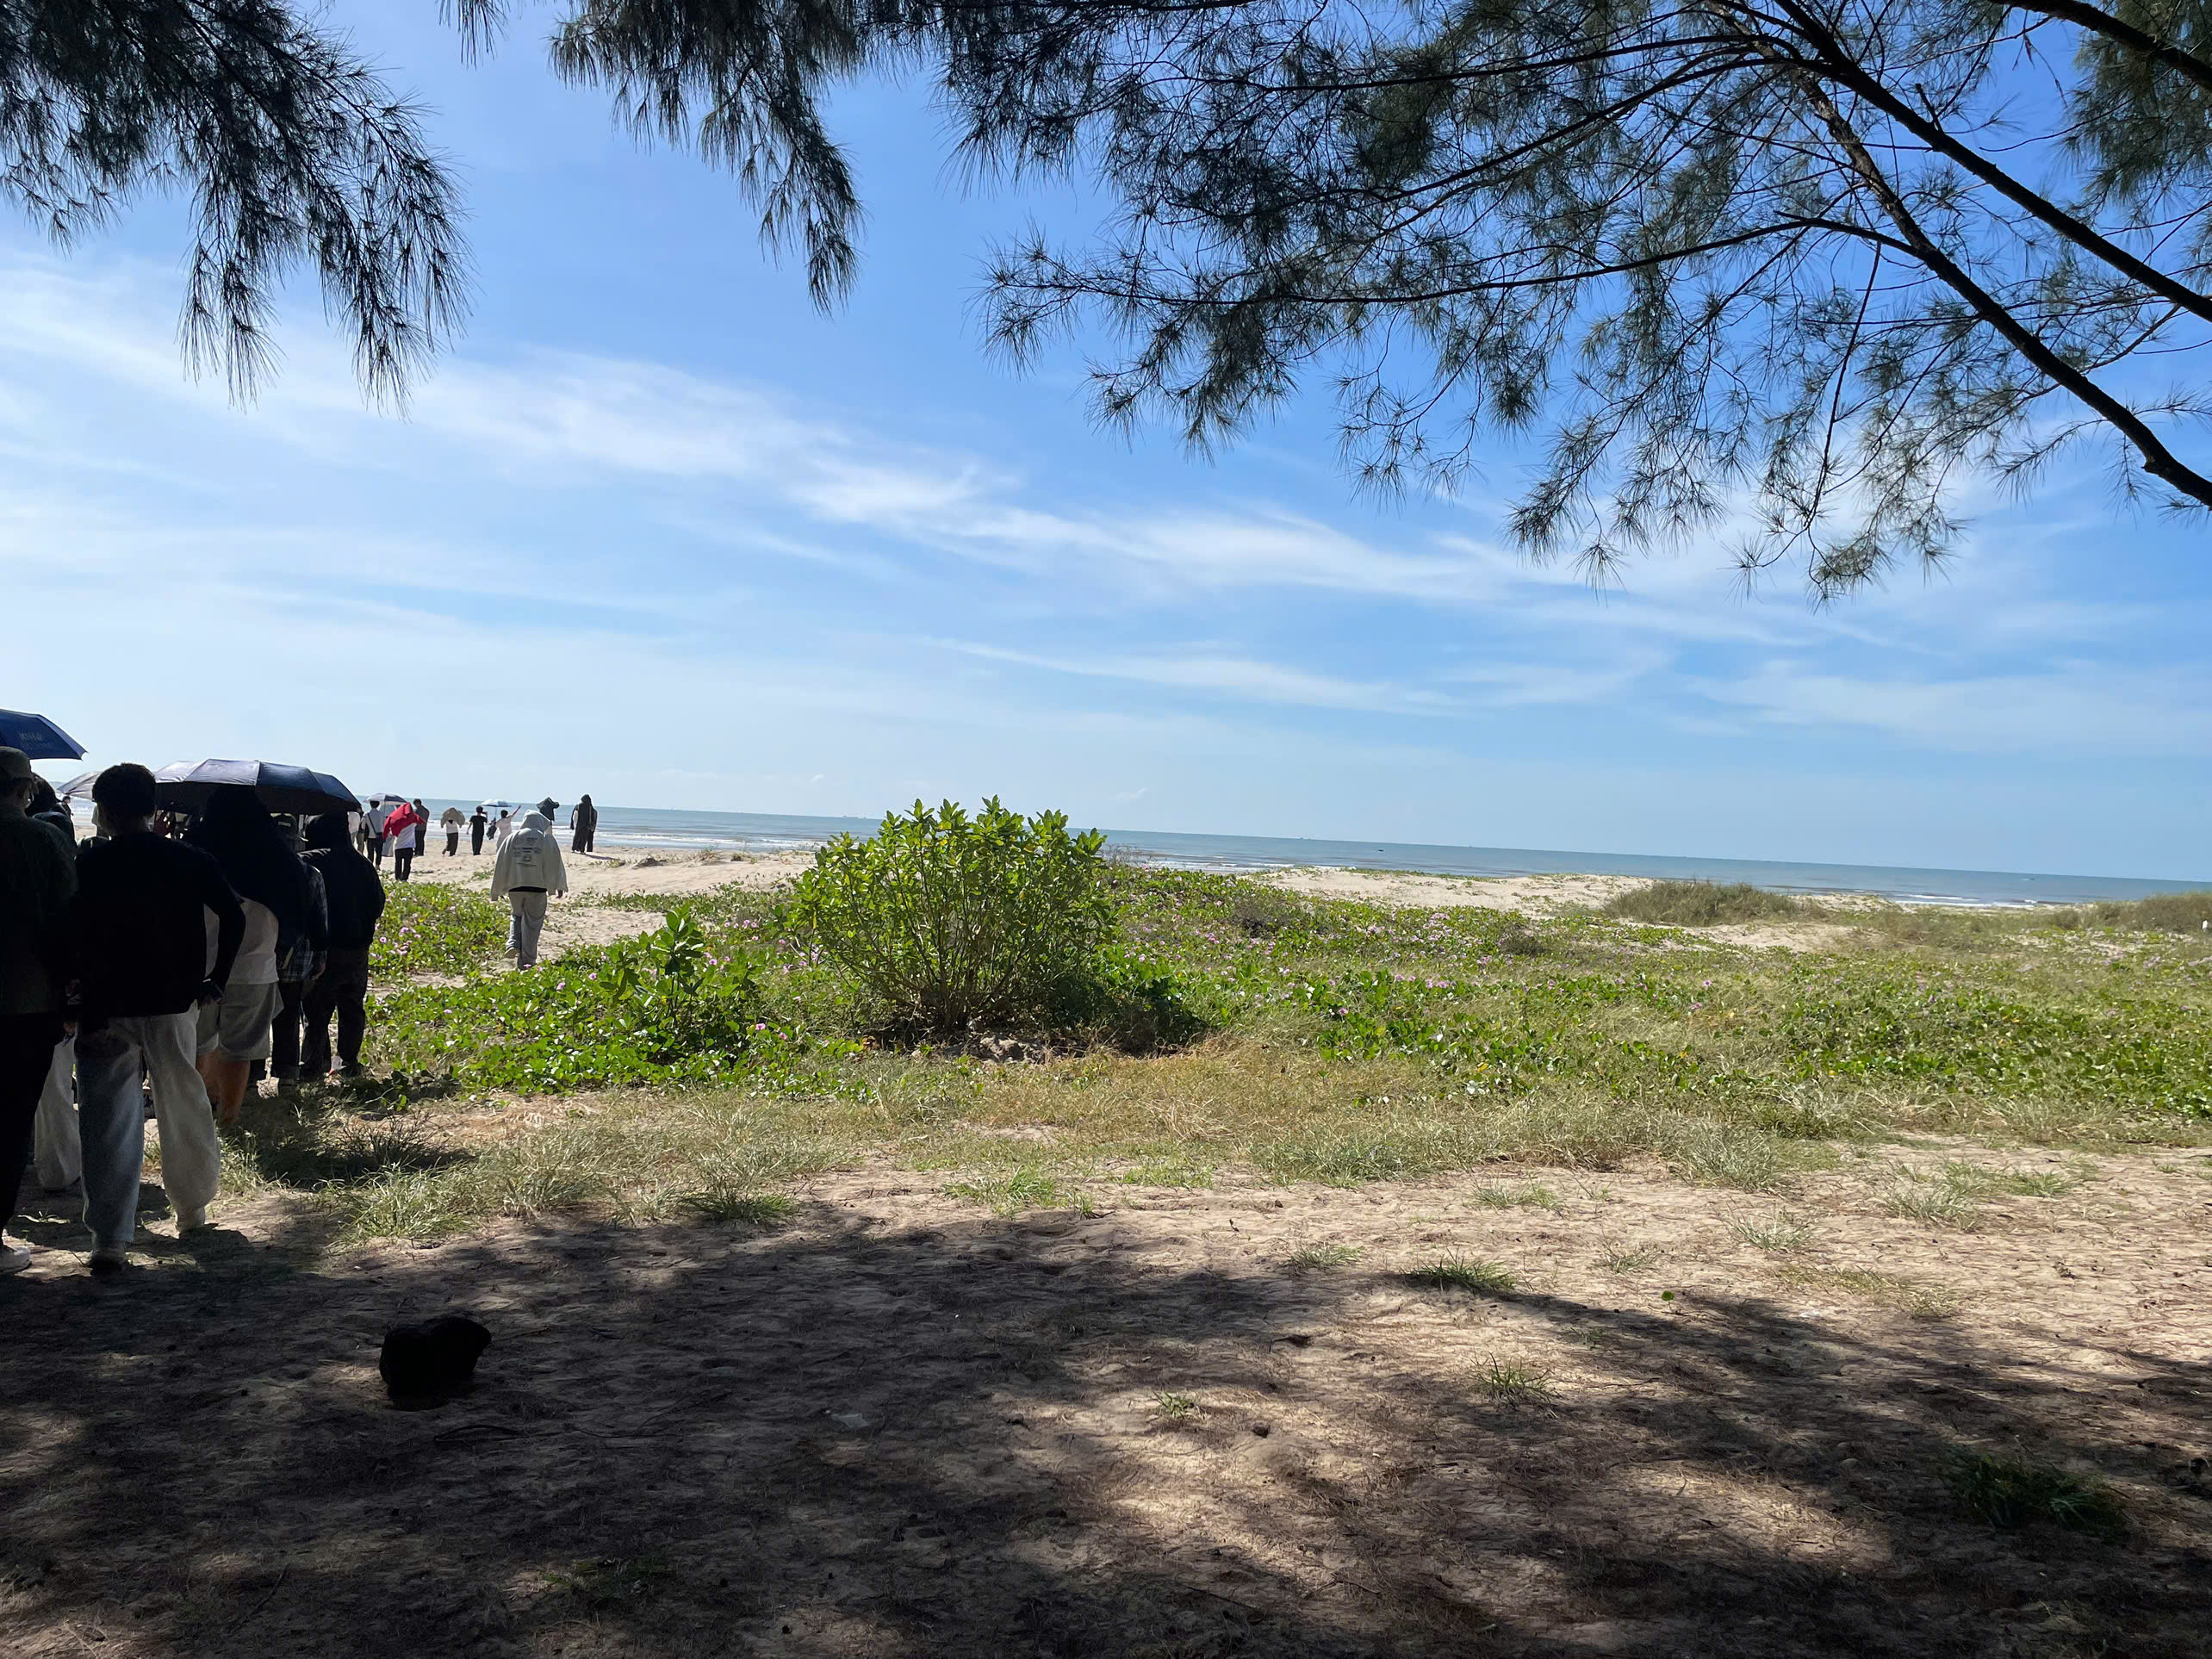
\includegraphics[width=0.8\textwidth]{images/groundwater_dunes.jpg}
    \caption{Aeolian sand dune surface acting as a groundwater recharge zone at Ho Tram.}
    \label{fig:groundwater_dunes}
\end{figure}

\subsection{Coastal Erosion, Wave Action, and Marine Processes (Back Beach, Mui Ke Ga, \& Ho Tram Estuary)}
Coastal hydrological processes were investigated across multiple distinct coastal environments, including Back Beach (Vung Tau), Mui Ke Ga, and the Ho Tram river mouth / coastal inlet (Cua Ho Tram).

At Back Beach and Cua Ho Tram, continuous wave action and tidal currents drive intense coastal sediment transport. High-energy waves strike the shoreline, creating steep beach scarps and eroding sandy shorelines, while longshore currents carry loose sand along the coast to form depositional bars near river inlets.

\begin{figure}[htbp]
    \centering
    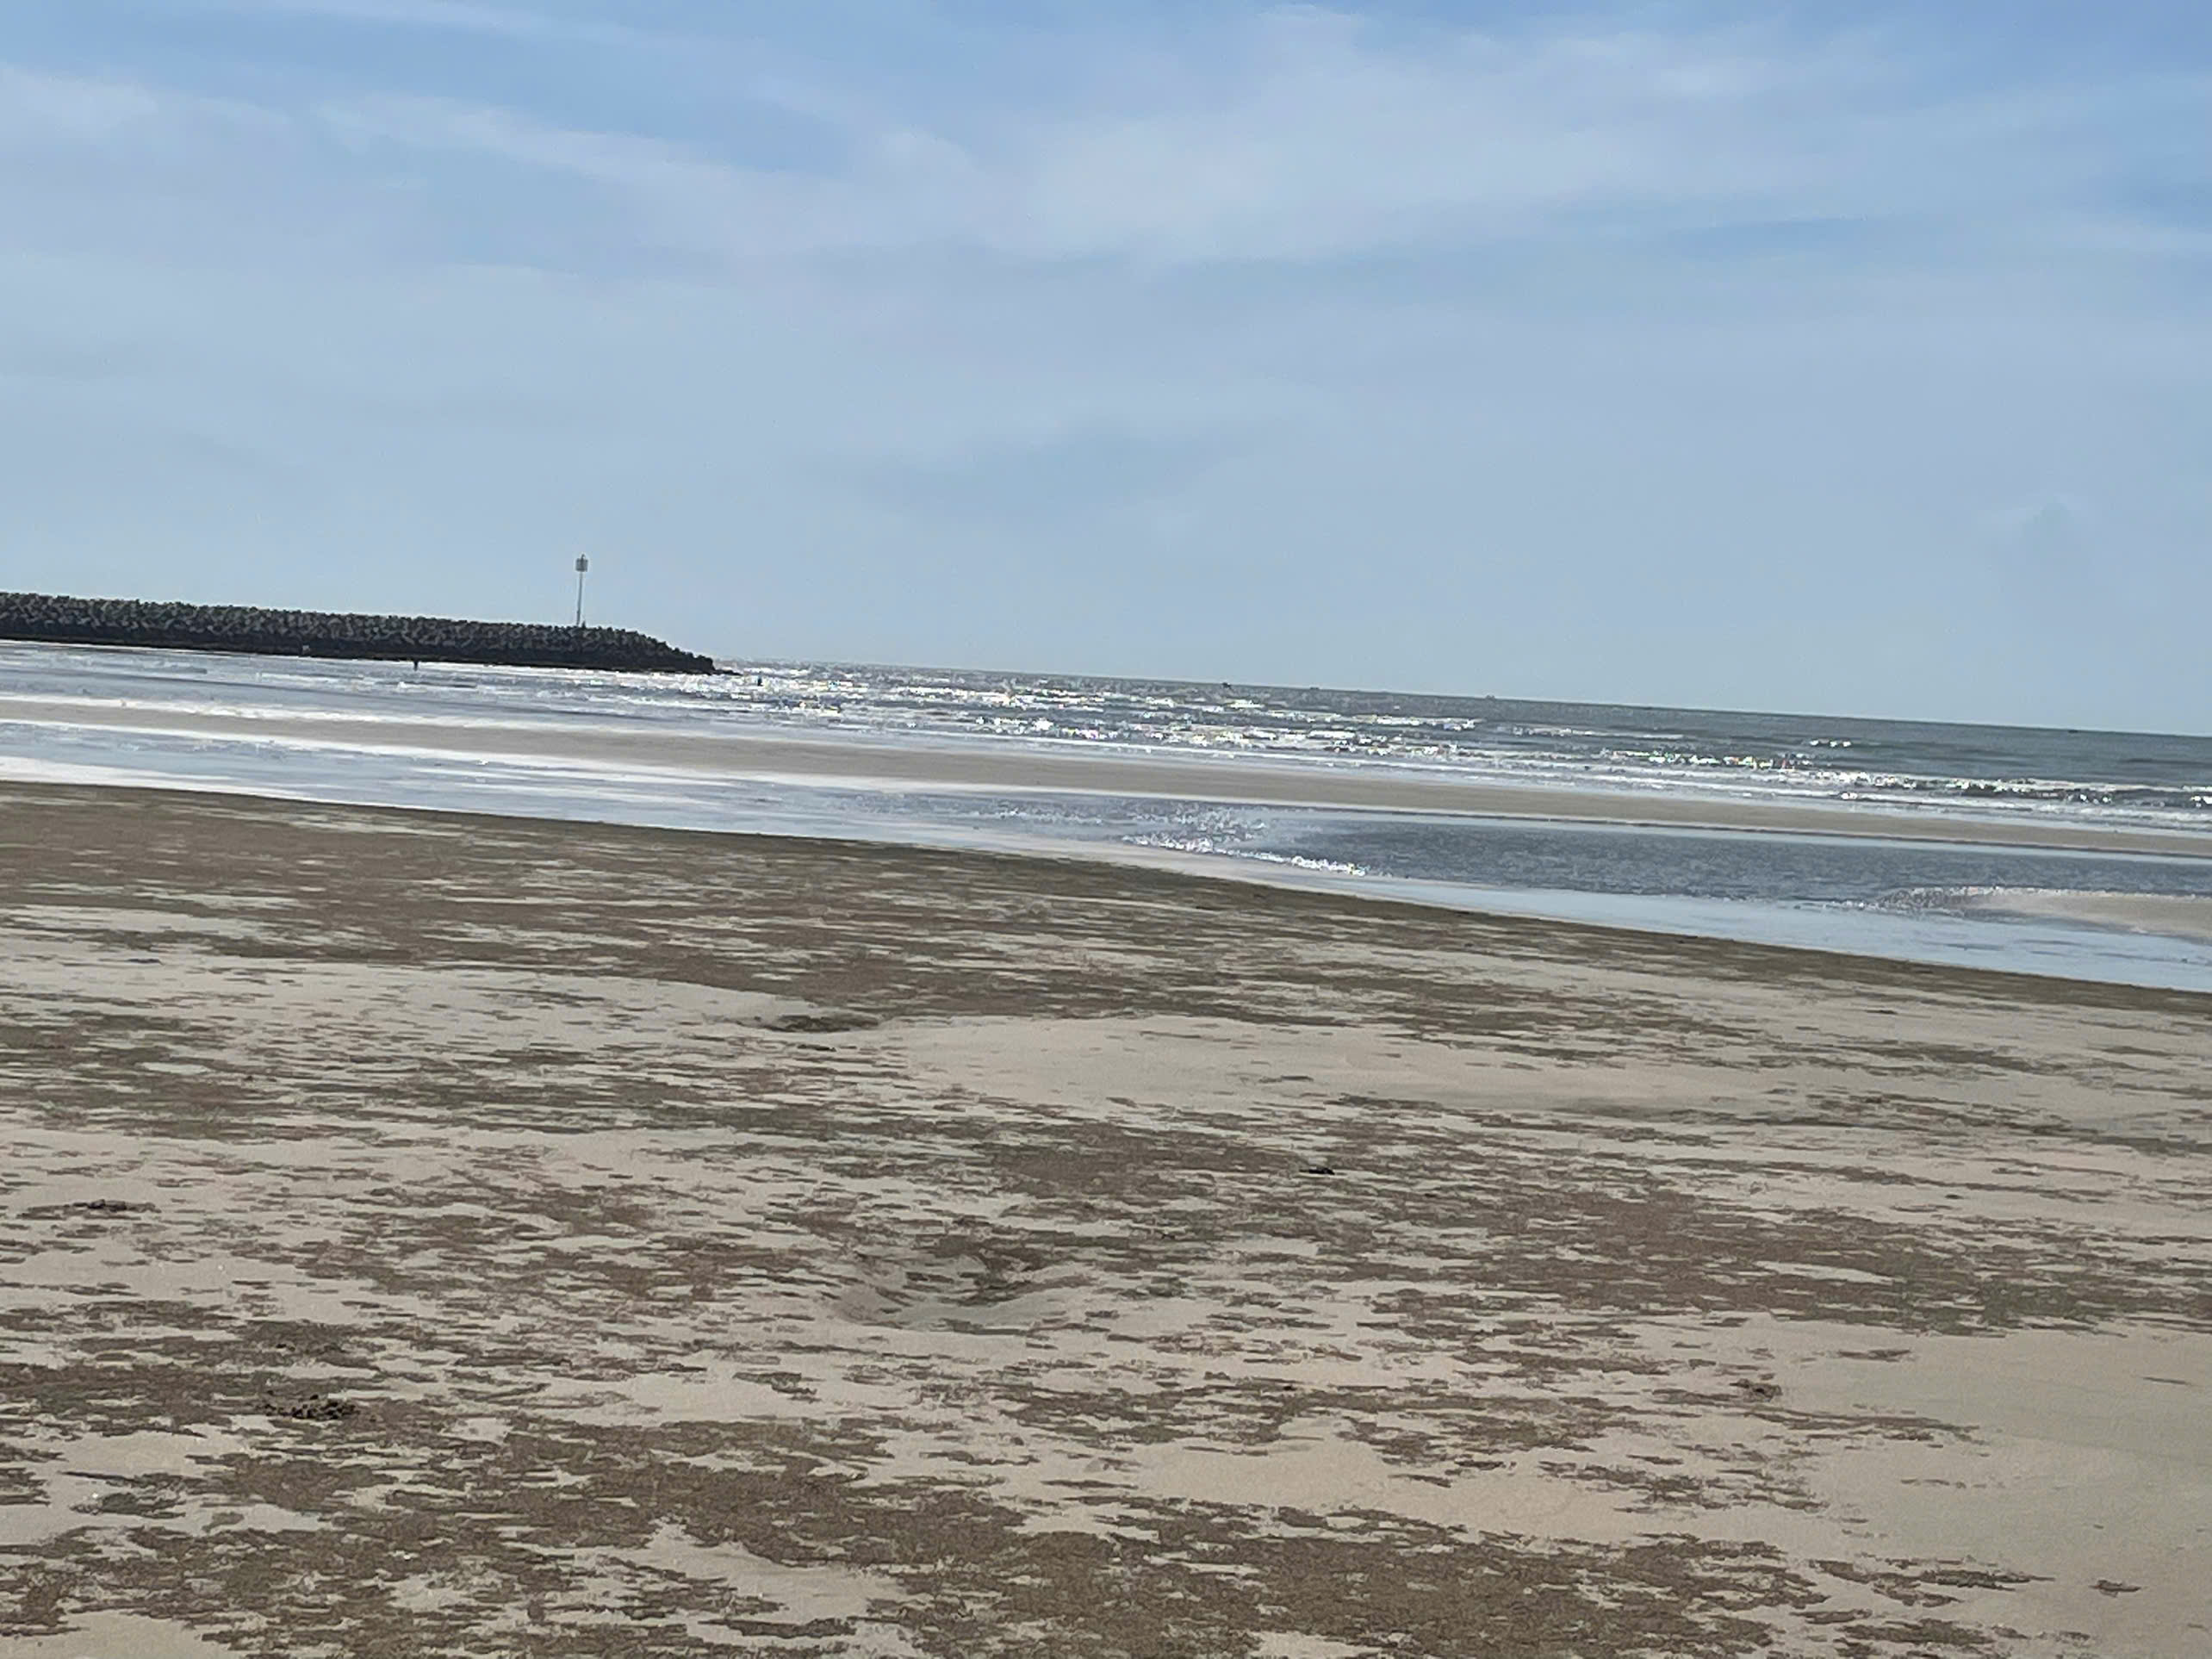
\includegraphics[width=0.8\textwidth]{images/coastal_erosion.jpg}
    \caption{Eroded sandy beach scarp and wave impact observed along the coast.}
    \label{fig:coastal_erosion}
\end{figure}

At Mui Ke Ga, where rocky headlands intersect the ocean, wave energy is concentrated directly against bedrock exposures. Mechanical wave battering and hydraulic fracturing constantly weather and erode the granitic headland structures, creating wave-cut platforms and sea cliffs. The contrasting dynamics between the sandy beaches of Ho Tram / Vung Tau and the rocky exposures of Mui Ke Ga highlight how coastlines respond differently to ocean hydrodynamics based on local geology.

\begin{figure}[htbp]
    \centering
    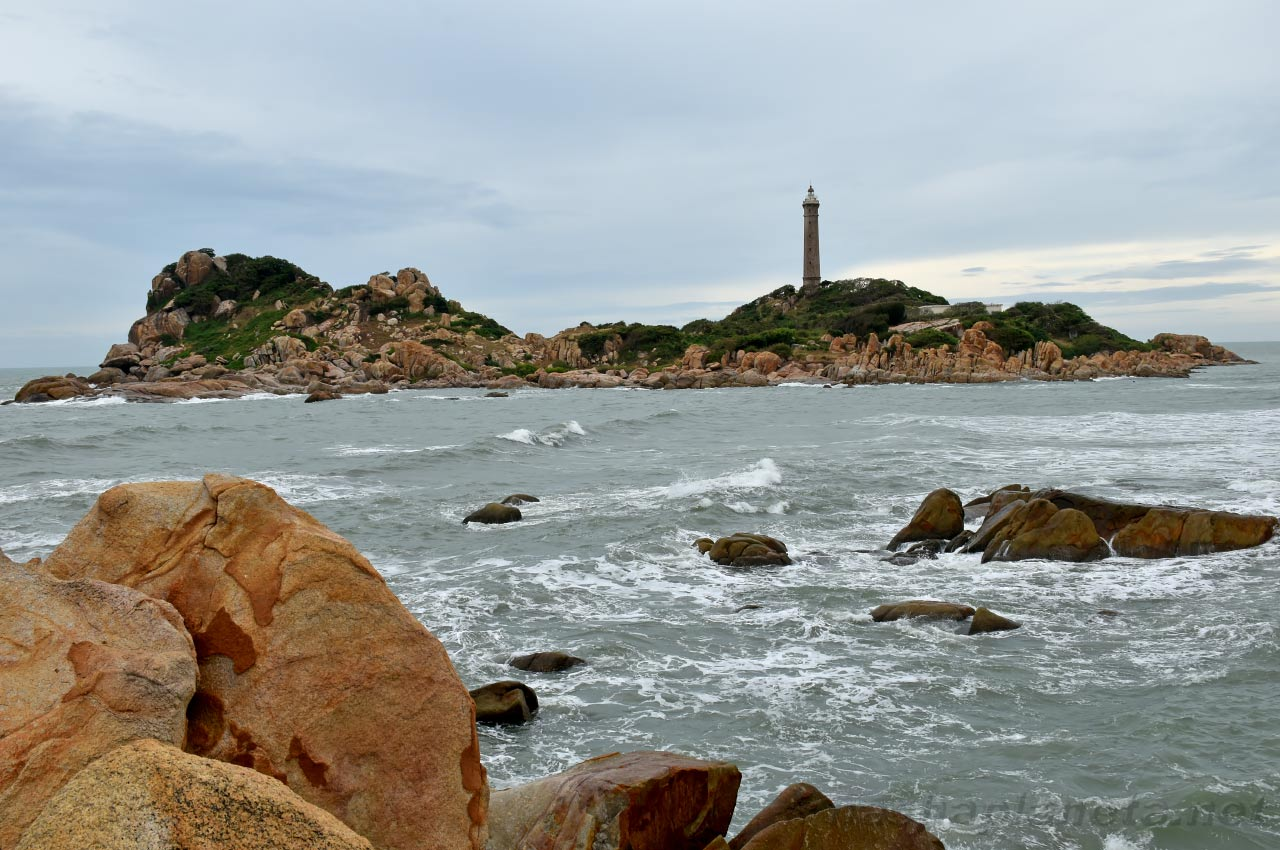
\includegraphics[width=0.8\textwidth]{images/ke_ga_coastal.jpg}
    \caption{Wave action against rocky granite headlands observed at Mui Ke Ga.}
    \label{fig:ke_ga_coastal}
\end{figure}

\subsection{Impact of Mining Pit Water Retention at Ho Da and Gia Quy Quarry}
The hydrosphere also interacts closely with human engineering and resource extraction activities, as observed at Ho Da (VNU-HCM Quarry lake) and Gia Quy Quarry.

At Ho Da, past quarrying deepened the basin below the regional water table, allowing groundwater seepage and surface runoff to accumulate over time. This created a permanent artificial quarry lake. Similarly, open-pit operations at Gia Quy Quarry alter local surface runoff paths and groundwater drainage. These sites demonstrate how anthropogenic excavations interrupt natural hydrological flow paths and create standing water bodies within former mining pits.

\begin{figure}[htbp]
    \centering
    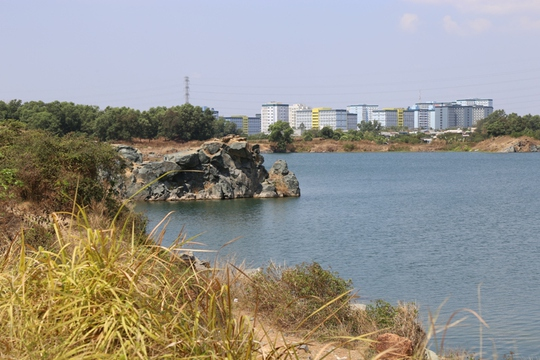
\includegraphics[width=0.8\textwidth]{images/ho_da_water.jpg}
    \caption{Accumulated surface and groundwater filling the former quarry pit at Ho Da.}
    \label{fig:ho_da_water}
\end{figure}

\section{Biosphere}

\subsection{Biological Weathering by Tree Roots}
Biological weathering is the breakdown of rocks caused by living organisms such as plants, roots, microorganisms, and animals. Among these agents, plant roots are one of the most common causes of biological weathering in exposed rock areas. When seeds fall into small cracks or fractures in rocks, they can germinate if there is enough moisture and soil material. As the plant grows, its roots gradually extend deeper into the fractures.

Over time, the roots become larger and exert pressure on the surrounding rock. This pressure slowly widens the cracks and weakens the rock structure. As a result, the rock may split into smaller blocks or fragments. This process is usually slow, but it is important because it contributes to the long-term breakdown of rocks at the Earth's surface.

During the fieldtrip, vegetation was observed growing along fractures in exposed rock. The plant stems and roots followed existing cracks in the rock surface. This observation shows how biological activity can take advantage of natural weaknesses in rocks and gradually enlarge them. The presence of vegetation also indicates that weathered material and moisture had accumulated in the cracks, allowing plants to grow.

\begin{figure}[htbp]
    \centering
    [Image: Plant growth along fractures]
    \caption{Plant growth along rock fractures, demonstrating biological weathering caused by roots.}
\end{figure}

This example demonstrates the connection between the biosphere and geosphere. The biosphere, represented by plant growth, directly affects the geosphere by weakening and breaking down rock materials. In addition, biological weathering can support other weathering processes. Once cracks become wider, more water and air can enter the rock, increasing chemical weathering and physical breakdown. Therefore, root growth plays an important role in rock weathering and landscape development.

\subsection{Mangrove Forests and Coastal Protection}
Mangrove forests are coastal ecosystems that commonly develop in river mouths, estuaries, tidal flats, and sheltered coastal zones. These environments are usually affected by brackish water, which is a mixture of freshwater from rivers and saltwater from the sea. Mangrove trees are specially adapted to muddy, wet, and saline environments. They often have dense root systems that help them survive in soft sediments and tidal conditions.

At river mouths, mangrove forests act as a natural transition zone between land and sea. Their root systems trap fine sediments carried by rivers and tides. As sediments accumulate around the roots, the ground becomes more stable. This process helps reduce sediment loss and supports the formation of coastal wetlands.

\begin{figure}[htbp]
    \centering
    [Image: Mangrove forest]
    \caption{Mangrove forest along a water channel, showing dense vegetation in a coastal wetland environment.}
\end{figure}

Mangrove forests play an important role in coastal protection. Their dense trunks, branches, and roots reduce the energy of waves, tidal currents, and storm surges before they reach inland areas. By slowing down water movement, mangroves help limit coastal erosion and protect riverbanks and shorelines. They also reduce the direct impact of strong winds and waves during storms.

In addition, mangroves provide habitats for many organisms, including fish, crabs, mollusks, birds, and microorganisms. Their root systems create sheltered environments where young aquatic animals can live and grow. Therefore, mangrove forests are important not only for coastal protection, but also for biodiversity and local ecosystems.

\begin{figure}[htbp]
    \centering
    [Image: Mangrove vegetation]
    \caption{Mangrove vegetation near a river-mouth environment, illustrating its role in stabilizing sediments and protecting coastal areas.}
\end{figure}

Although mangrove forests were not the main focus of every field observation, they are highly relevant to the Earth system because they show the interaction between the biosphere, hydrosphere, and geosphere. Mangrove vegetation grows in coastal water environments, traps sediments, stabilizes shorelines, and reduces erosion. Therefore, mangrove forests are natural barriers that help protect coastal areas from waves, storms, and flooding.

\section{Atmosphere}

The coastal route from Vung Tau to Phan Thiet provides an opportunity to relate regional climate to the landscapes studied during the fieldtrip. Rainfall seasonality, atmospheric moisture, and wind help explain the conditions under which exposed rocks weather and loose coastal sediments are reworked.

\subsection{Climatic Characteristics of Vung Tau}

Vung Tau has a warm climate throughout the year, with a clear seasonal distribution of rainfall. The climatic data published in QCVN 02:2022/BXD give an annual mean air temperature of 27.1\,$^{\circ}$C and annual rainfall of approximately 1,419\,mm at Vung Tau station. Most rainfall occurs from May to October, while the first months of the year are much drier. Annual mean relative humidity is approximately 80\%~\cite{climate-qcvn}.

This seasonal pattern provides context for the coastal environments visited at Bai Sau and the Loc An coastal site (Cua Ho Tram). Rain supplies moisture to exposed soils and fractured rock, while subsequent drying changes the condition of surface materials. Warm, moist conditions support chemical weathering where water can react with minerals. At sandy sites, alternating wet and dry conditions also influence the availability of loose grains for wind transport. The atmosphere therefore contributes to landscape development through both the supply of water and the movement of air.

\begin{figure}[H]
    \centering
    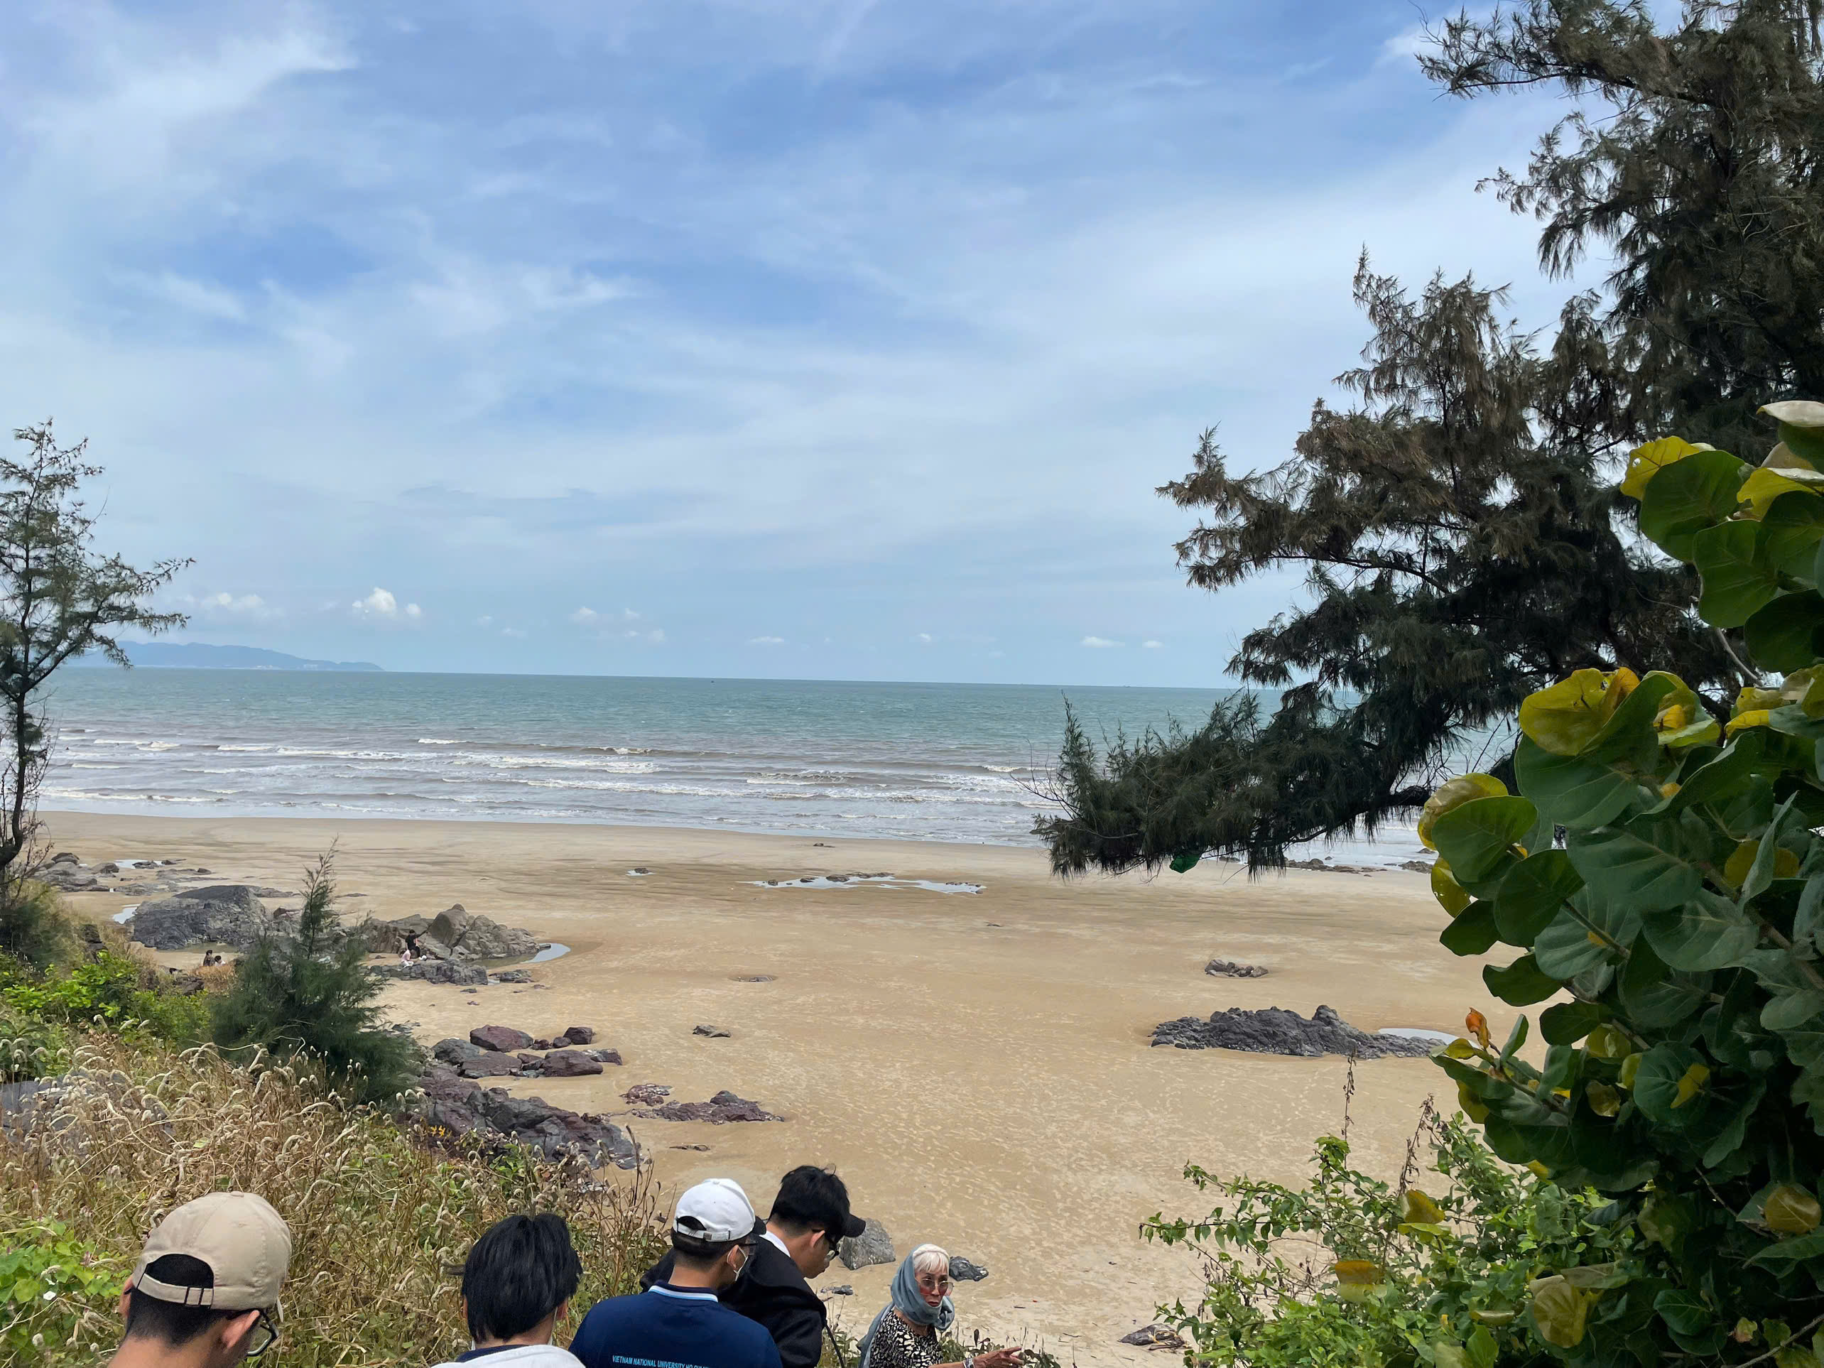
\includegraphics[width=0.82\textwidth]{images/bai_sau_atmosphere.png}
    \caption{Coastal setting at Bai Sau during the fieldtrip, showing the sky, sandy beach, exposed rocks, and shoreline vegetation.}
    \label{fig:atmosphere_bai_sau}
\end{figure}

\subsection{Climatic Characteristics of Phan Thiet and Their Landscape Significance}

Phan Thiet is also warm throughout the year, but receives less annual rainfall than Vung Tau. The same national dataset reports an annual mean temperature of 26.9\,$^{\circ}$C and annual rainfall of approximately 1,089\,mm at Phan Thiet station~\cite{climate-qcvn}. The city's 2023 land-use planning report describes a rainy season from approximately mid-May to late October and a dry season from November to April, together with around 2,600--2,700 hours of sunshine annually~\cite{climate-phanthiet}. These figures indicate that the regional contrast is particularly evident in rainfall availability, while annual mean temperatures remain similar.

For the sand-rich landscapes around Mui Ne, including the surroundings of Suoi Tien, this climatic setting helps explain the importance of surface drying and wind action. When sand is exposed, sufficiently dry, and not protected by vegetation, wind can move grains by short hops and rolling, producing erosion and deposition. The amount of sand moved depends on wind strength, sediment supply, surface moisture, and vegetation cover~\cite{wind-transport}. The balance between rainfall, surface drying, and wind exposure therefore helps determine when loose sand is available for transport.

\begin{figure}[H]
    \centering
    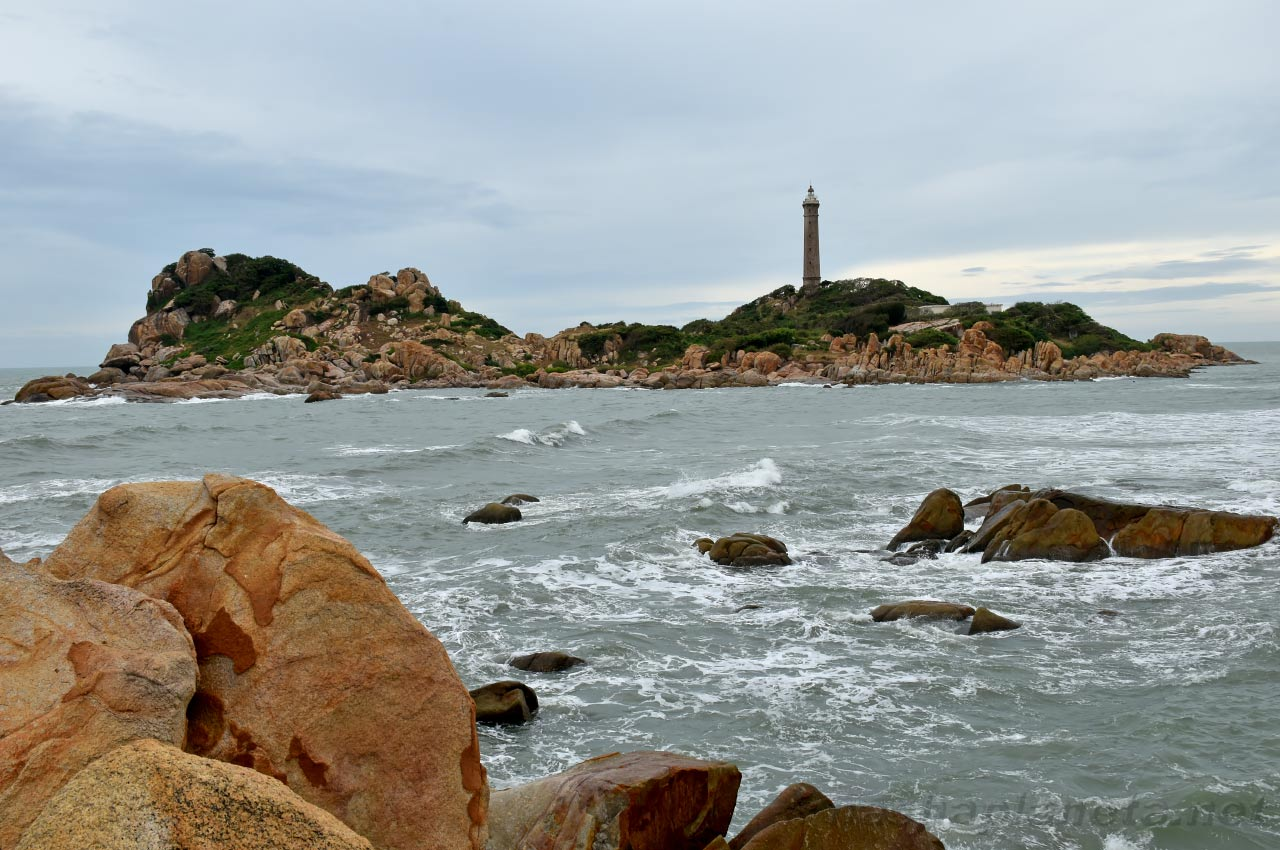
\includegraphics[width=0.82\textwidth]{images/ke_ga_coastal.jpg}
    \caption{Coastal setting at Mui Ke Ga, showing a cloudy sky above the rocky shoreline and lighthouse.}
    \label{fig:atmosphere_ke_ga}
\end{figure}

\section{Natural Resources}

The resource-related stops helped us examine how geological materials become useful products and how extraction changes the surrounding environment. Ho Da and Gia Quy provided examples of construction-stone resources at different stages of land use, while Vietsovpetro introduced the engineering systems required to develop offshore petroleum resources. Together, these sites connected resource availability with material quality, technical choices, economic efficiency, and responsibility for the landscape left after extraction. The rock examples discussed below are selected illustrations from the wider survey, including andesite at Ho Da, basalt at Gia Quy, and granite at Mui Ke Ga.

\subsection{Construction Stone and the Post-mining Landscape at Ho Da}

Ho Da, within the VNU-HCM area, is a former quarry where the remaining excavation has become a lake. The exposed rock, water surface, and vegetation visible around the site show how a landscape continues to change after the principal extraction activity has ended. From a resource perspective, the most important feature is the excavation itself: construction stone has been removed, leaving a landform whose future use must account for the geometry of the remaining rock faces and the presence of water.

At Ho Da, our field notes identify andesite as one of the rocks examined. This provides a specific example of the geological material exposed at the former quarry~\cite{group-field-notes}. Removing stone changes the ground surface and the setting for water and vegetation, so the resulting landscape forms part of the assessment of resource development.

The usefulness of construction stone depends on material quality as well as the quantity available. Competent igneous rock can supply aggregates, but weathered, fractured, porous, or altered portions of a deposit may behave differently from fresh rock. Geological assessment consequently examines variations across an exposure and relates them to the intended use. Properties such as particle size, strength, water absorption, and durability require appropriate evaluation before a material is selected for a particular construction application~\cite{aggregate-geology}. The exposures at Ho Da provide a field setting in which to discuss this connection between geological condition and engineering performance.

\begin{figure}[H]
    \centering
    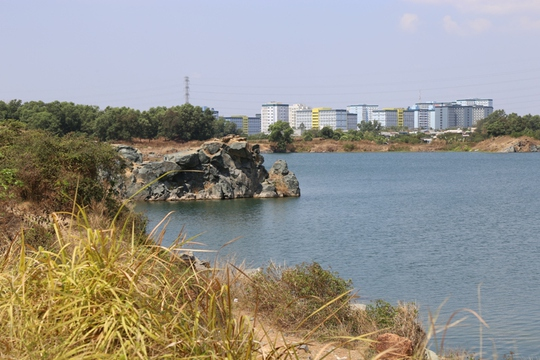
\includegraphics[width=0.82\textwidth]{images/ho_da_water.jpg}
    \caption{The post-mining landscape at Ho Da, with a water-filled excavation, exposed rock faces, and vegetation around the lake.}
    \label{fig:resources_ho_da}
\end{figure}

Vegetation around the lake shows that plant growth can return to disturbed ground. However, assessing a former quarry also requires examining the remaining highwalls and changes in drainage and groundwater conditions. Research on abandoned quarry highwalls emphasizes that slope assessment must continue to consider conditions after extraction stops~\cite{quarry-highwalls}. The presence of plants and water is therefore only part of the information needed to evaluate a post-mining landscape.

A rehabilitation plan should link the physical condition of the site to a realistic future use. Possible measures include stabilizing slopes, reshaping disturbed ground where appropriate, managing drainage, and establishing vegetation~\cite{quarry-ehs}. For Ho Da, the educational value of exposed rock and the landscape can be considered alongside the management of access and steep edges. The lesson from this stop is that responsible resource use includes both obtaining a useful material and planning for the land after that material has been removed.

\subsection{Construction Stone Resources and Quarry Engineering at Gia Quy}

The group examined a range of rocks and minerals at Gia Quy; the discussion and photographs below present a few illustrative examples. Our field notes describe basalt, including compact and vesicular varieties, and weathered rock with brown surfaces and fractures~\cite{group-field-notes}. The field photographs show exposed quarry faces, accumulations of broken rock, and a material-handling area. Seeing these features together helped connect the rock mass in an exposure with material that can enter the construction supply chain. The quarry face represents the source, while the detached fragments and handling facilities illustrate subsequent stages in using that source.

Basalt and other suitable igneous rocks can be processed into crushed stone~\cite{aggregate-geology}. In the aggregate industry, extracted material is crushed and sorted into sizes appropriate for its application; it may then be used directly or combined with cement or asphalt to produce construction materials~\cite{aggregate-uses}. The Gia Quy visit provided a practical setting for understanding why a natural rock resource needs selection and processing before it becomes a usable product.

\begin{figure}[H]
    \centering
    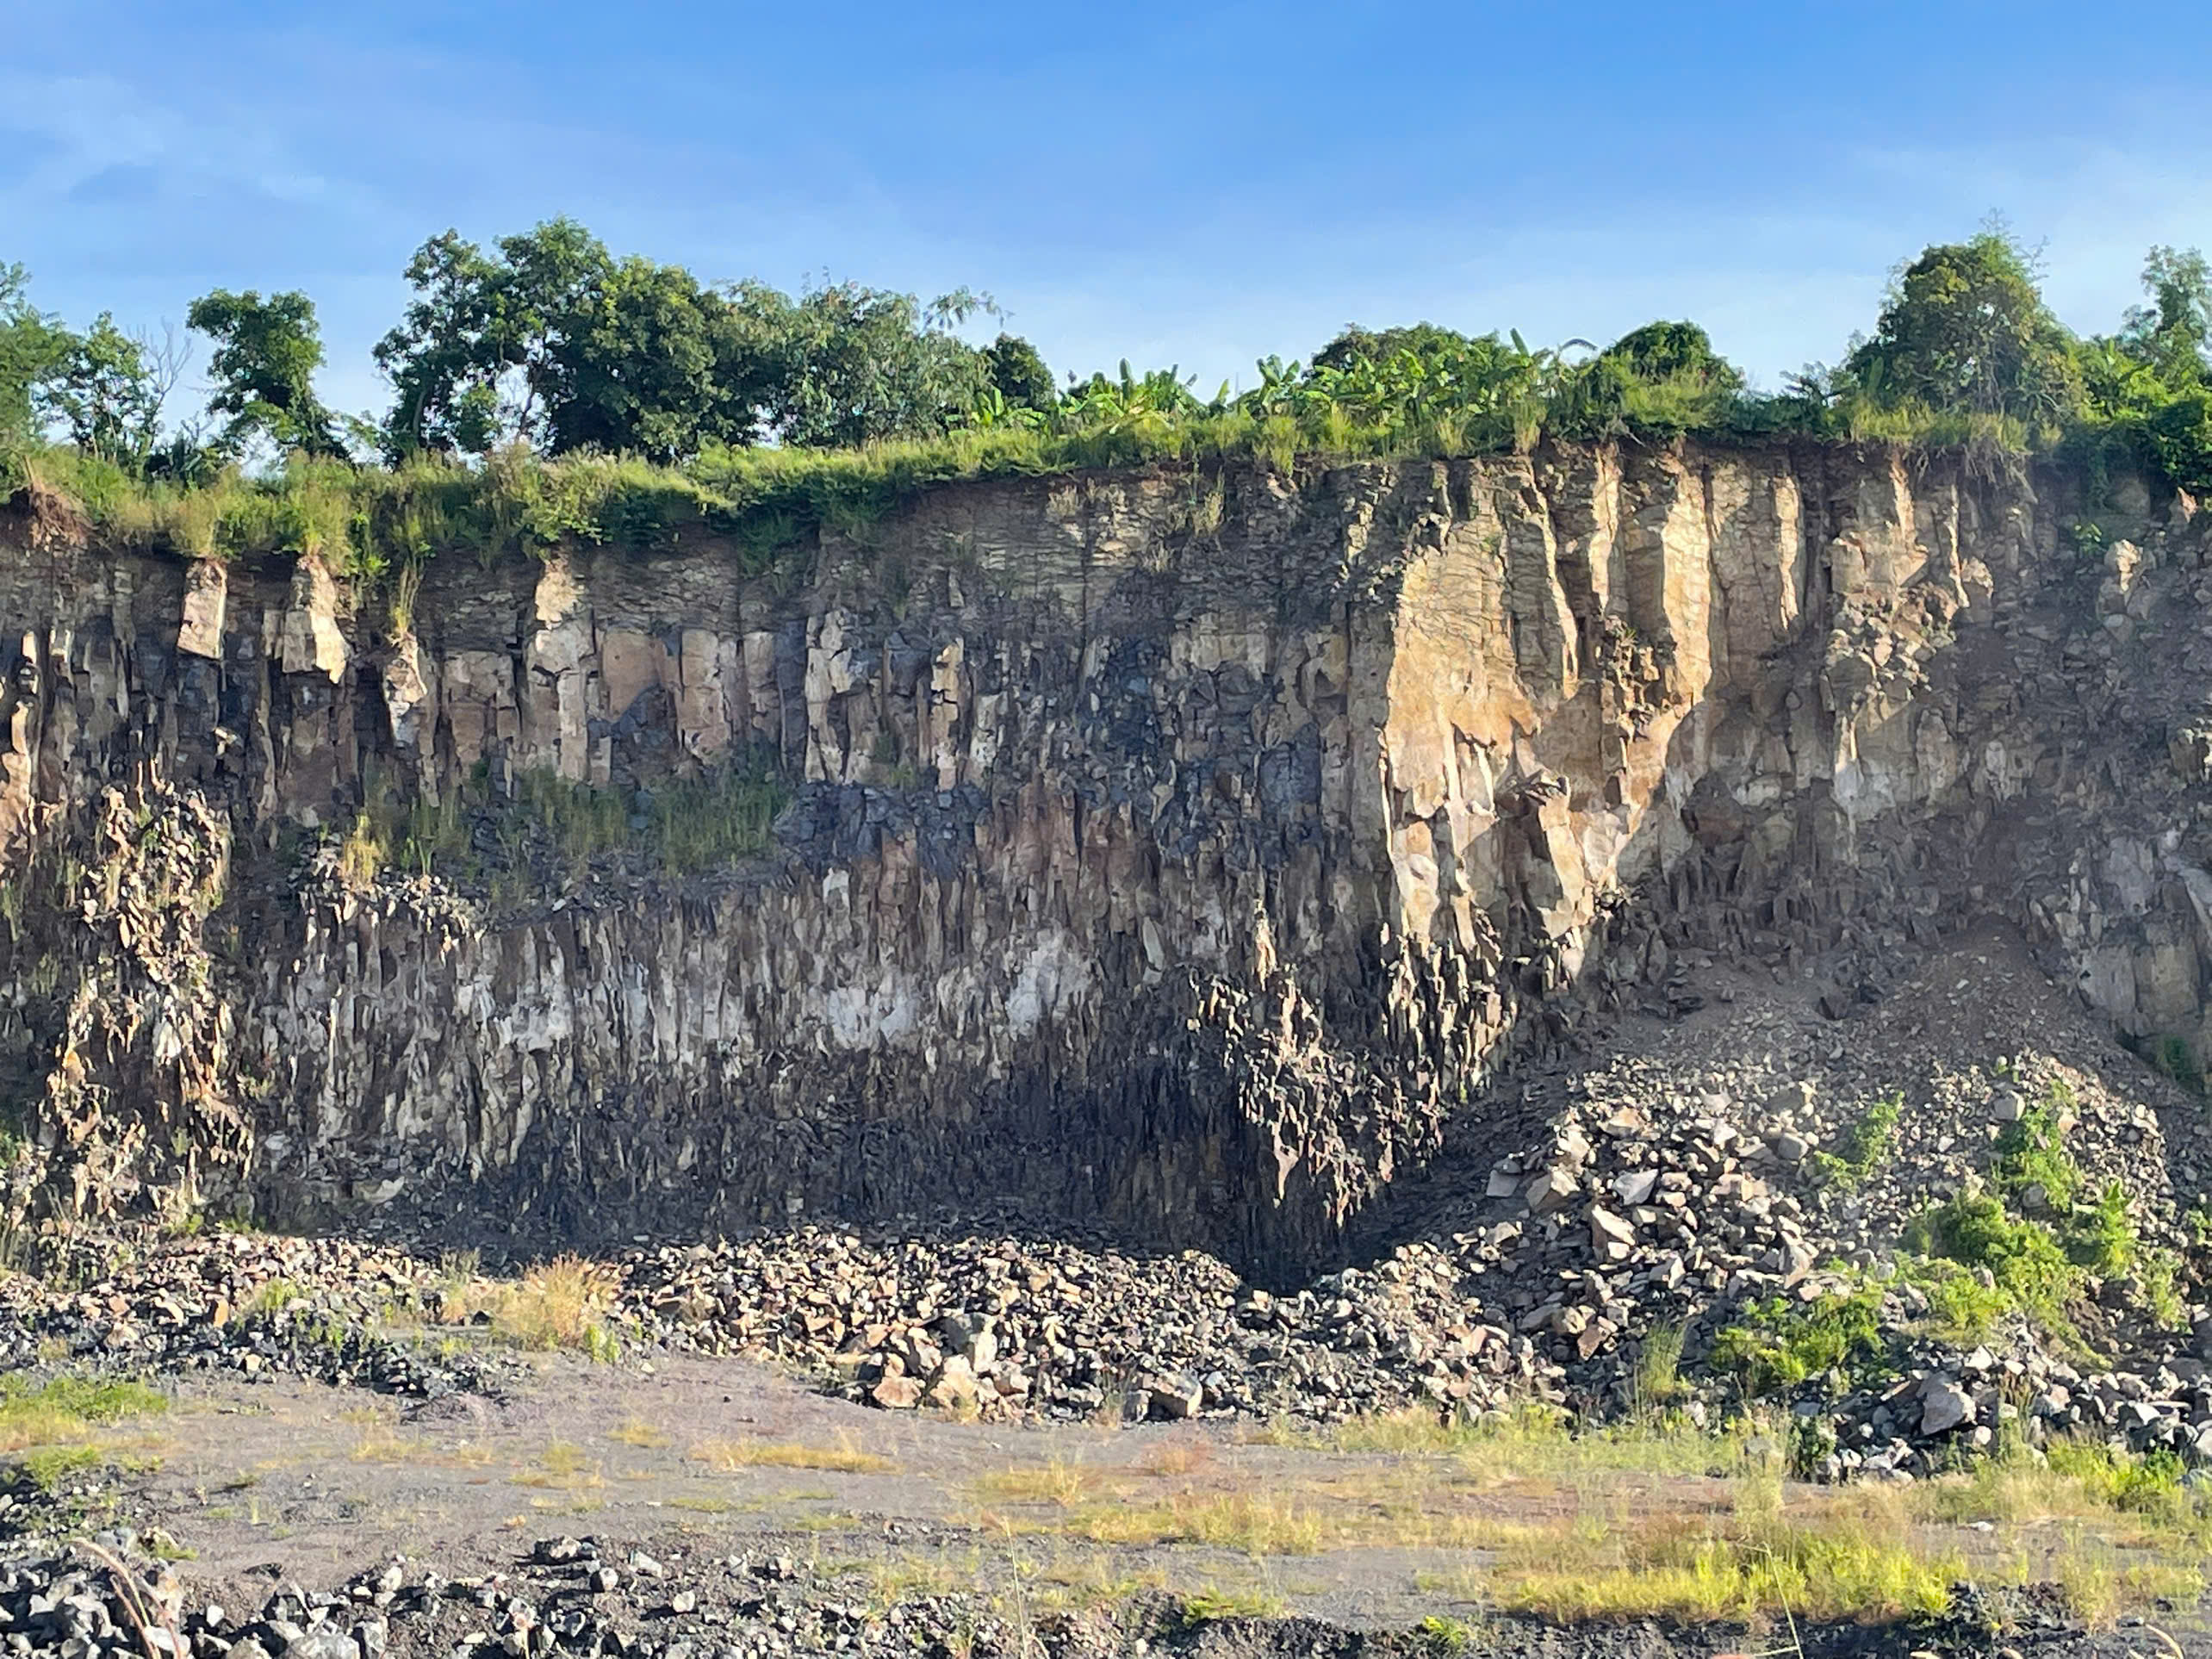
\includegraphics[width=0.66\textwidth]{images/gia_quy_mat_mo.jpg}
    \caption{Quarry face at Gia Quy, showing fractured rock and accumulated fragments at the foot of the exposure.}
    \label{fig:resources_gia_quy_face}
\end{figure}

The fractures visible in the quarry face are relevant to both extraction and the condition of the remaining rock mass. Their influence must be considered together with the shape of the excavation and changes in groundwater and surface drainage. Quarry highwall research connects extraction methods and site conditions with both short-term and long-term slope behaviour~\cite{quarry-highwalls}. Thus, the economic value of a rock deposit cannot be separated from the engineering work needed to access it.

In a quarry layout, benches, drainage, and routes for equipment help organize extraction and movement of material~\cite{quarry-ehs}. These are applications of geological and geotechnical knowledge to an excavation. The exposed face and broken blocks made this connection between resource extraction and excavation design visible at the site.

\begin{samepage}
Two selected specimens illustrate some of the mineralogical features discussed during the visit: an olivine-bearing rock and a white calcite specimen. The first contained green olivine in a dark host rock. Olivine is an iron--magnesium silicate, commonly represented by $(Mg,Fe)_2SiO_4$, and occurs in basalt and other igneous rocks. A separate white specimen was identified as calcite, a calcium-carbonate mineral with the formula $CaCO_3$~\cite{field-minerals}. These examples showed a contrast between a silicate mineral within a rock and a carbonate mineral specimen.

\end{samepage}

The samples helped us distinguish the mineralogical interest of an occurrence from the economic assessment of a deposit. Recognizing an individual mineral adds information about a site, while evaluating a construction-stone resource also requires considering the amount, continuity, and engineering quality of the usable material.

\begin{figure}[H]
    \centering
    \begin{minipage}[t]{0.31\textwidth}
        \vspace{0pt}
        \centering
        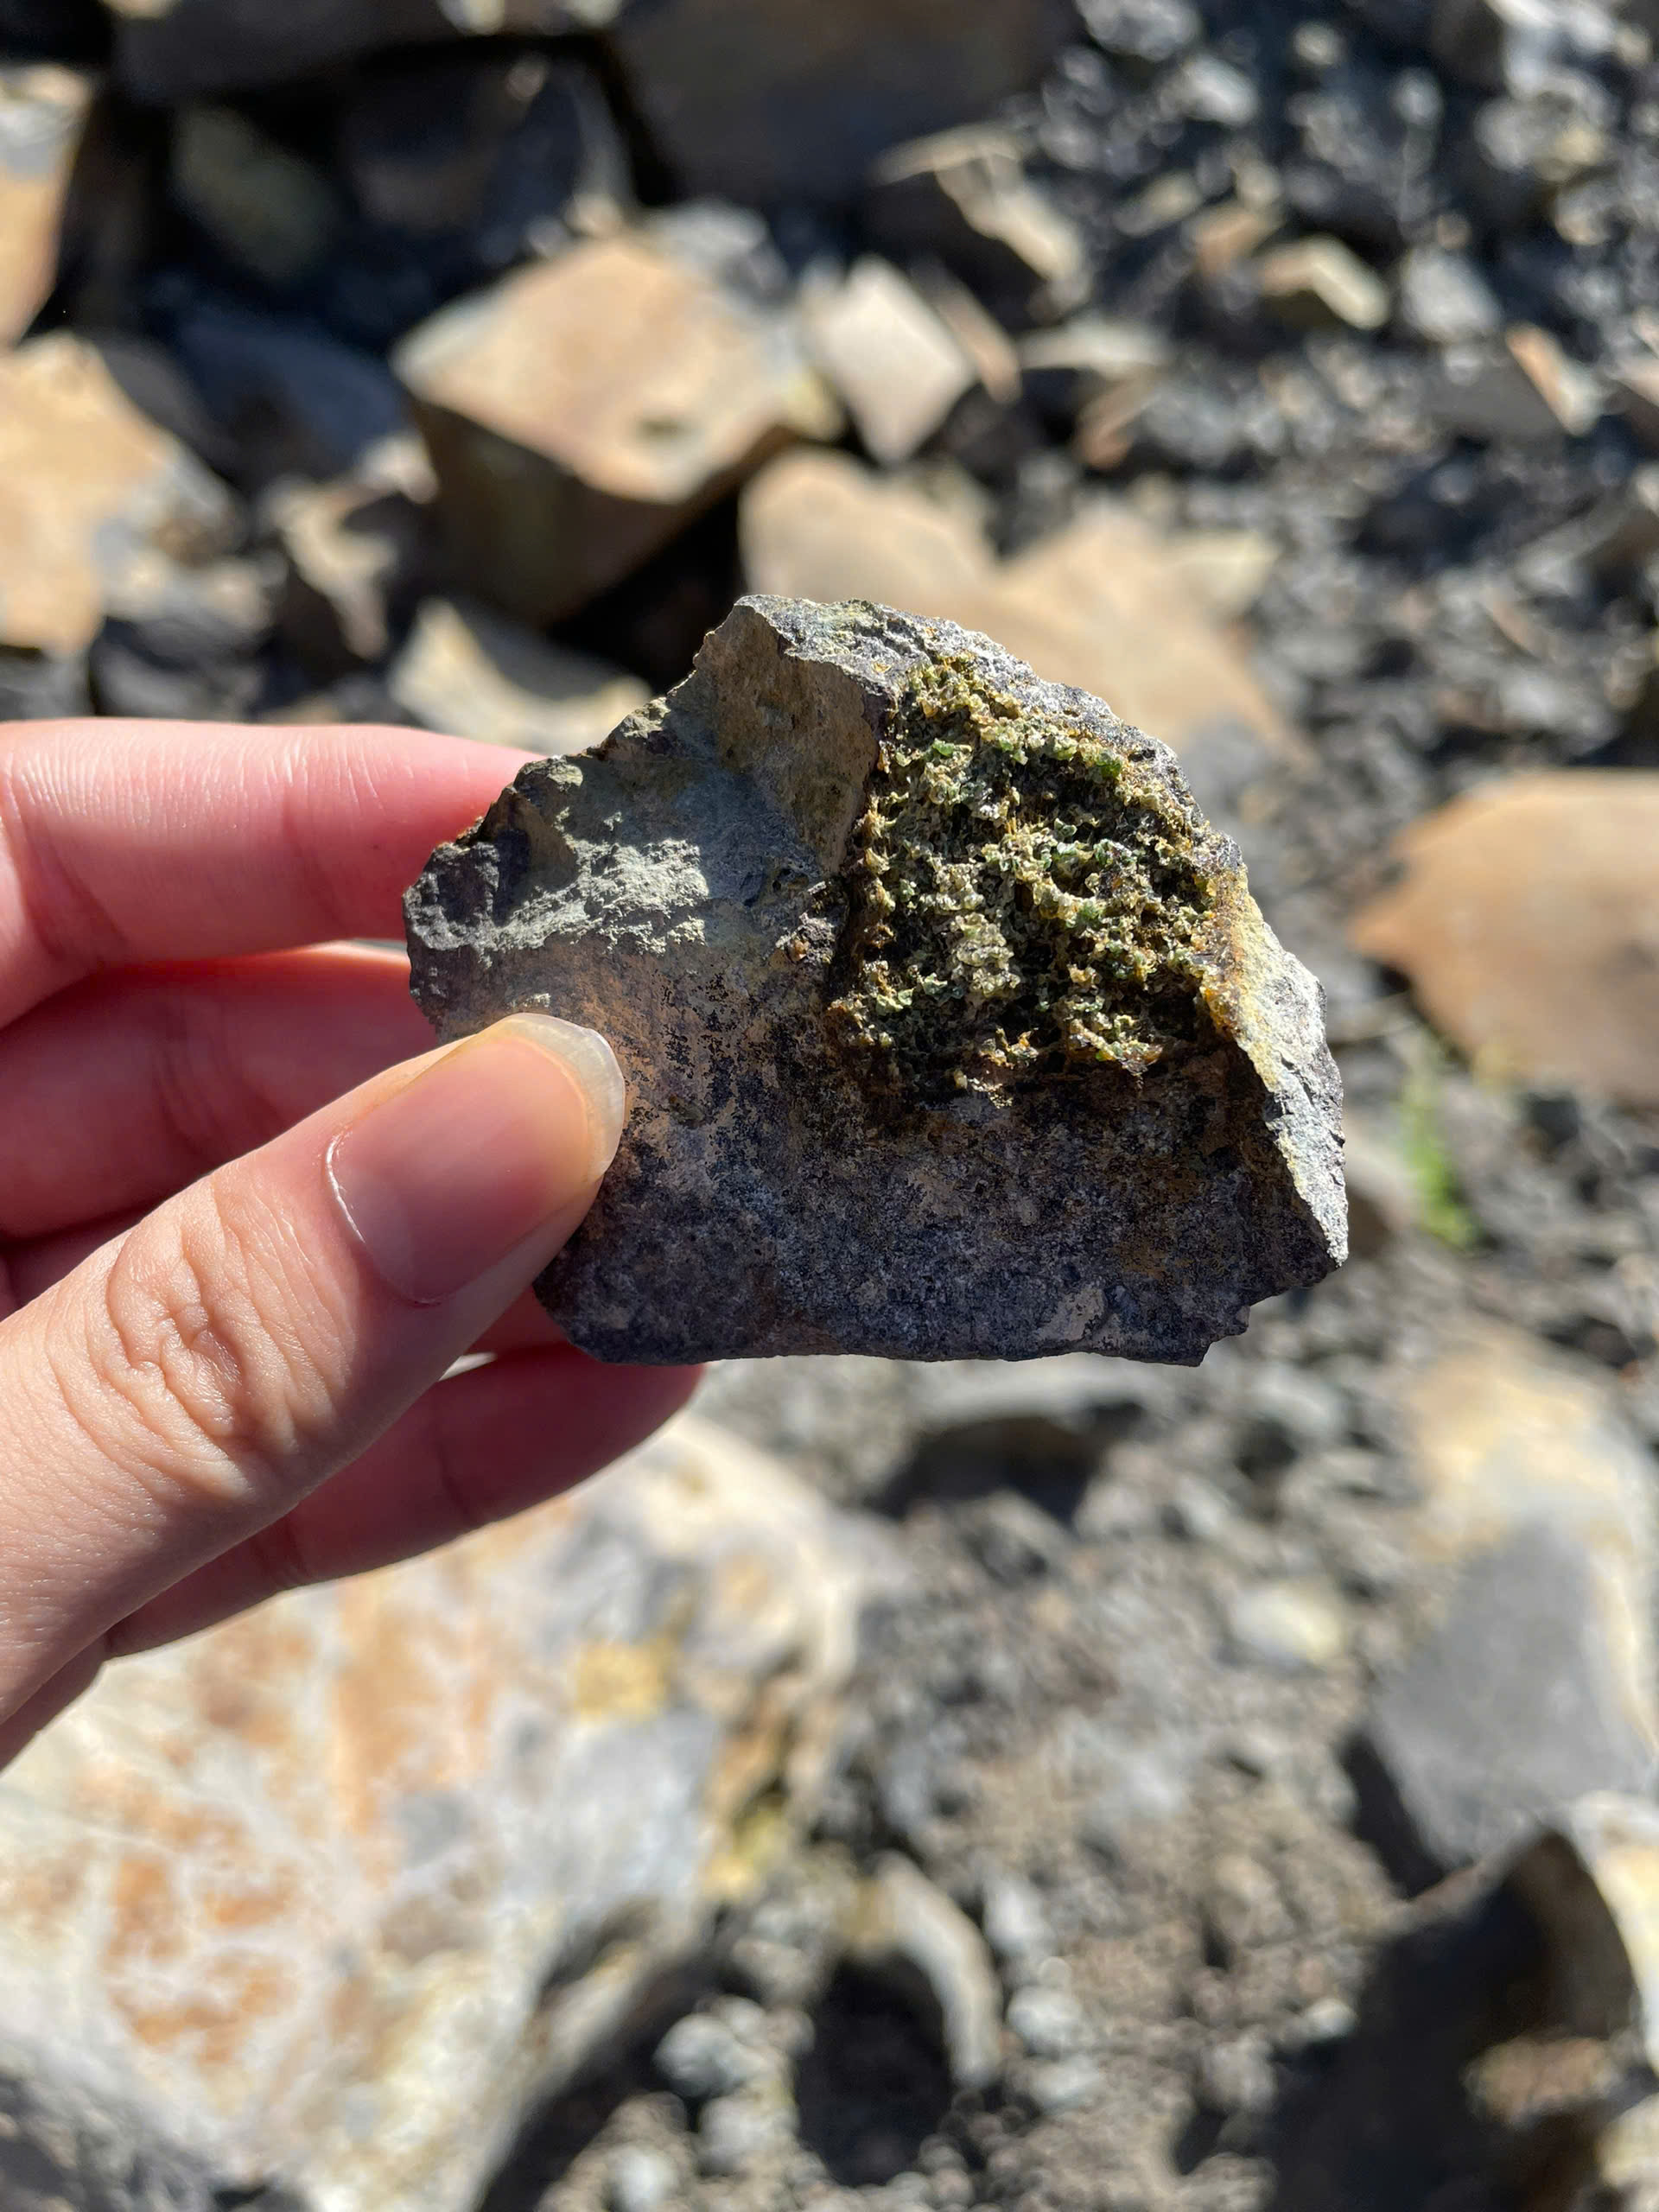
\includegraphics[width=\linewidth,height=3.8cm,keepaspectratio]{images/gia_quy_mau_olivine.jpg}
    \end{minipage}\hfill
    \begin{minipage}[t]{0.31\textwidth}
        \vspace{0pt}
        \centering
        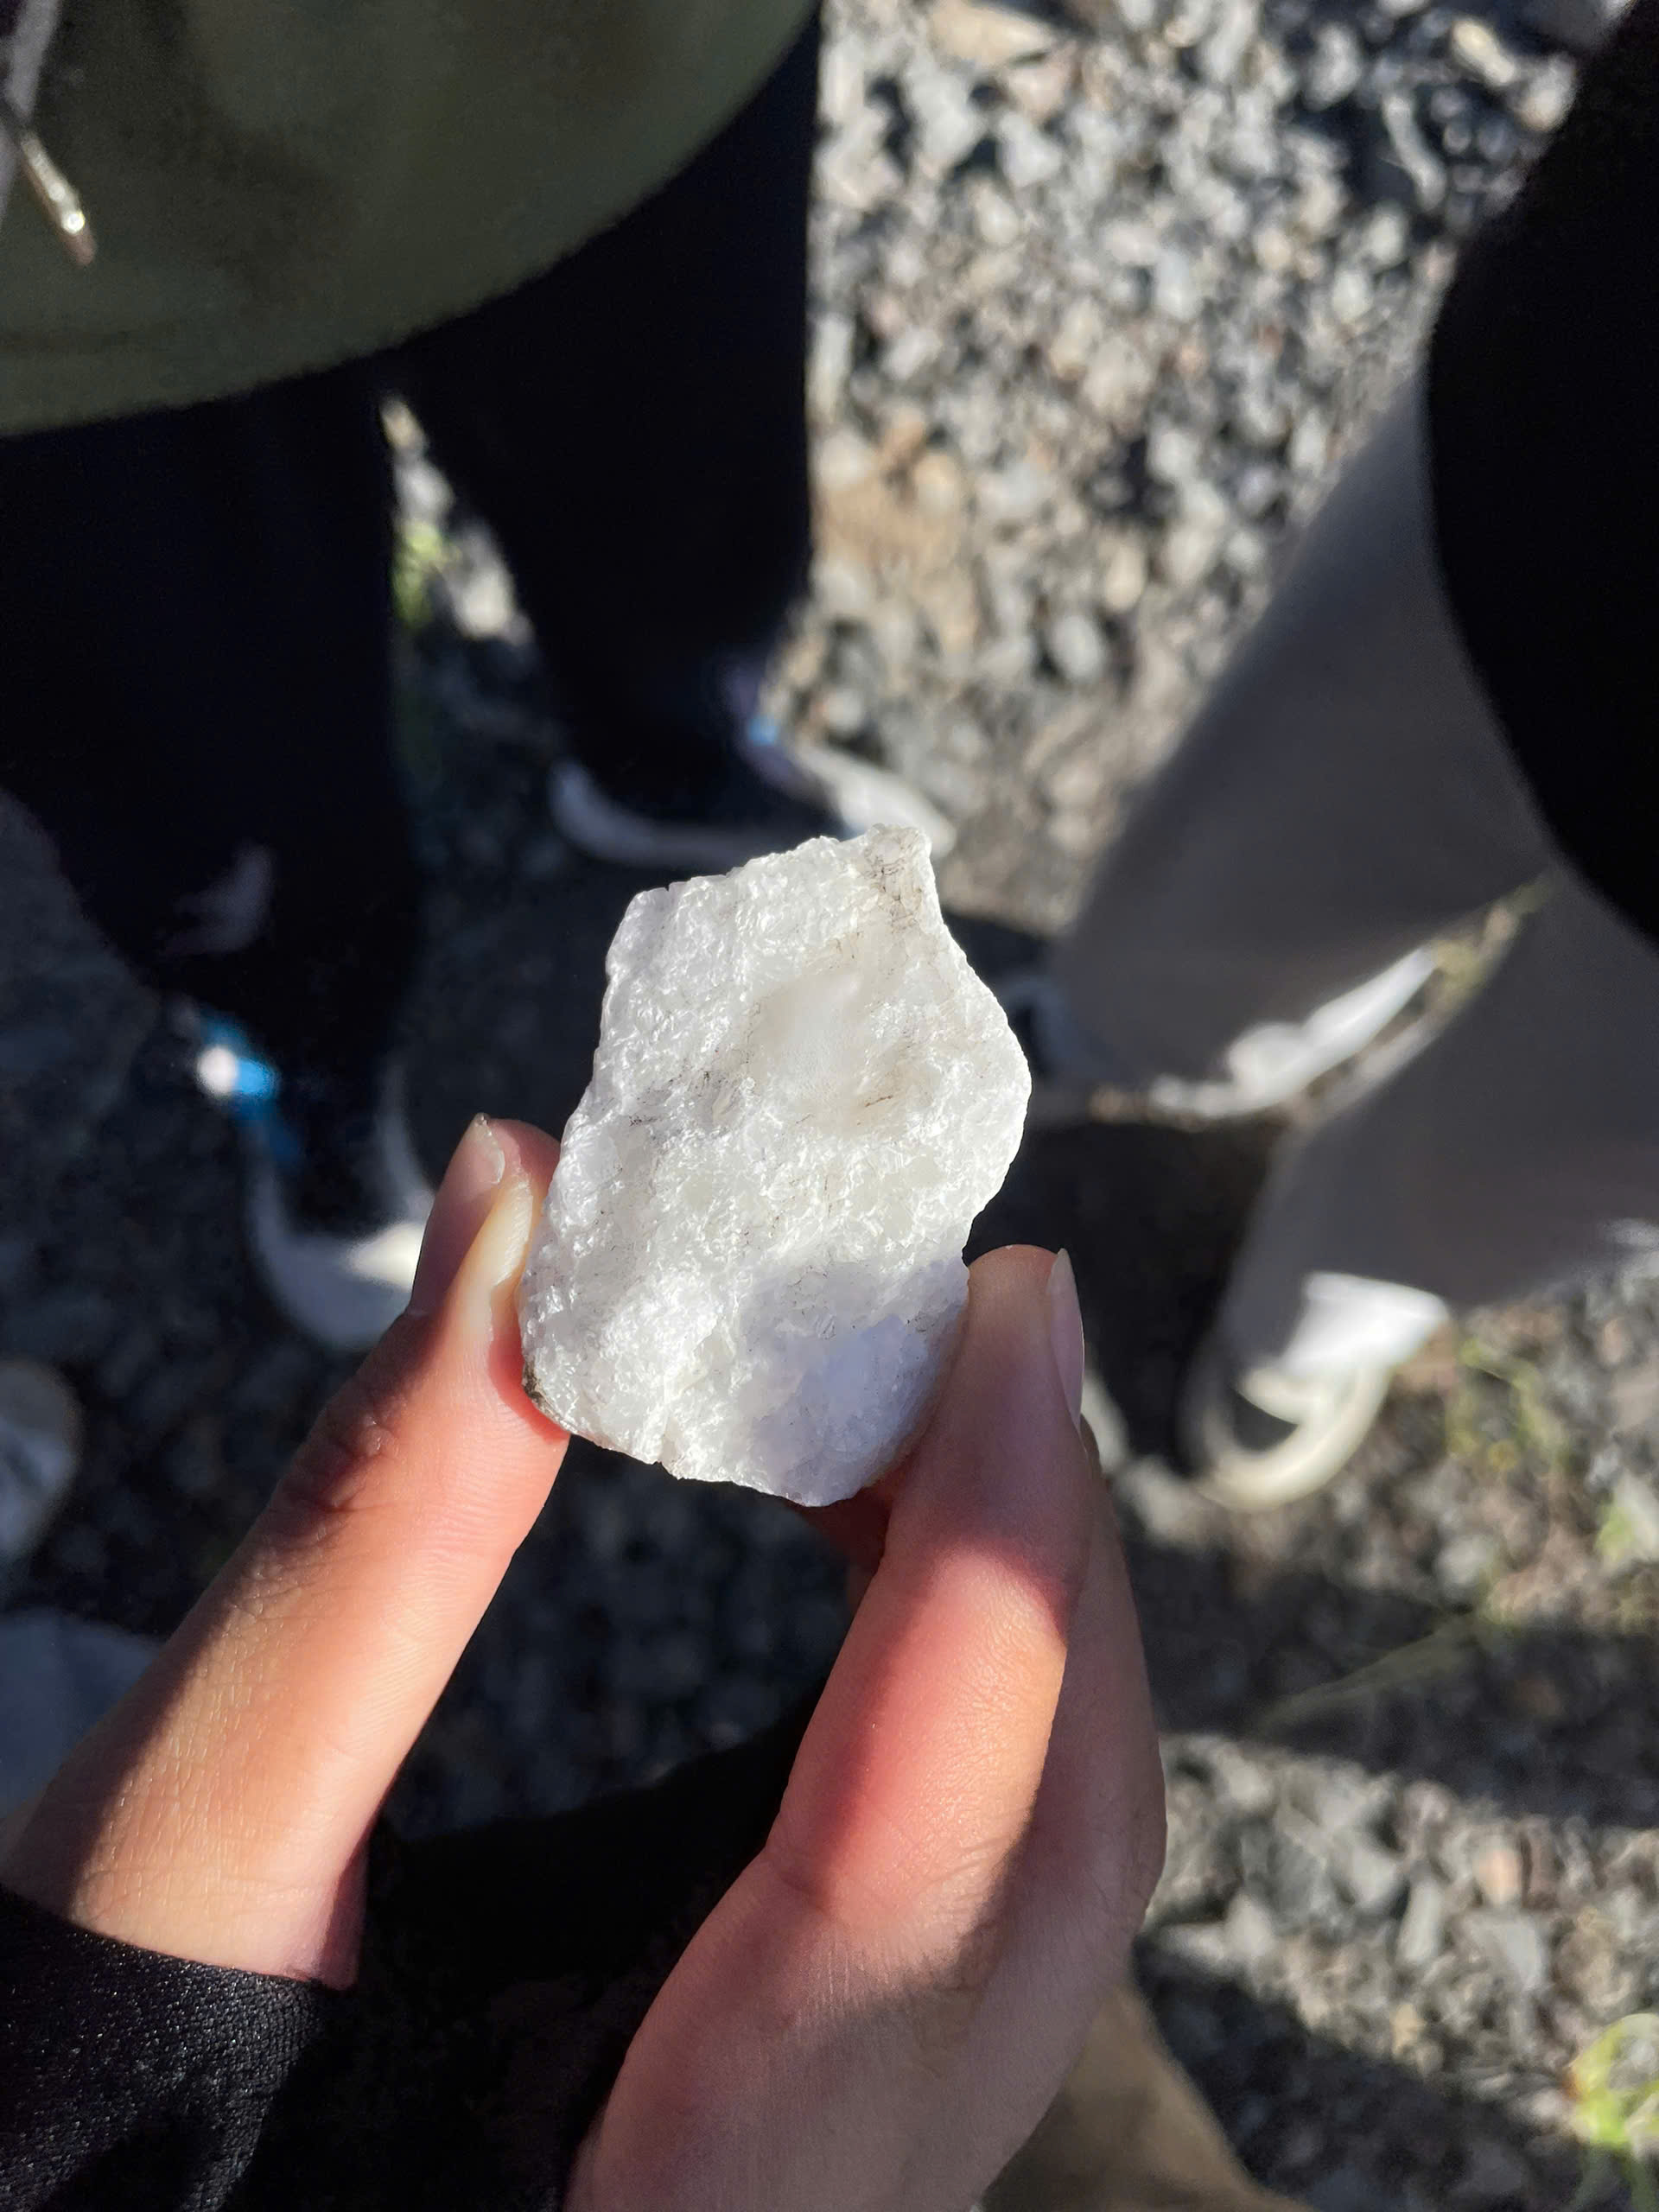
\includegraphics[width=\linewidth,height=3.8cm,keepaspectratio]{images/gia_quy_mau_canxit.jpg}
    \end{minipage}\hfill
    \begin{minipage}[t]{0.31\textwidth}
        \vspace{0pt}
        \centering
        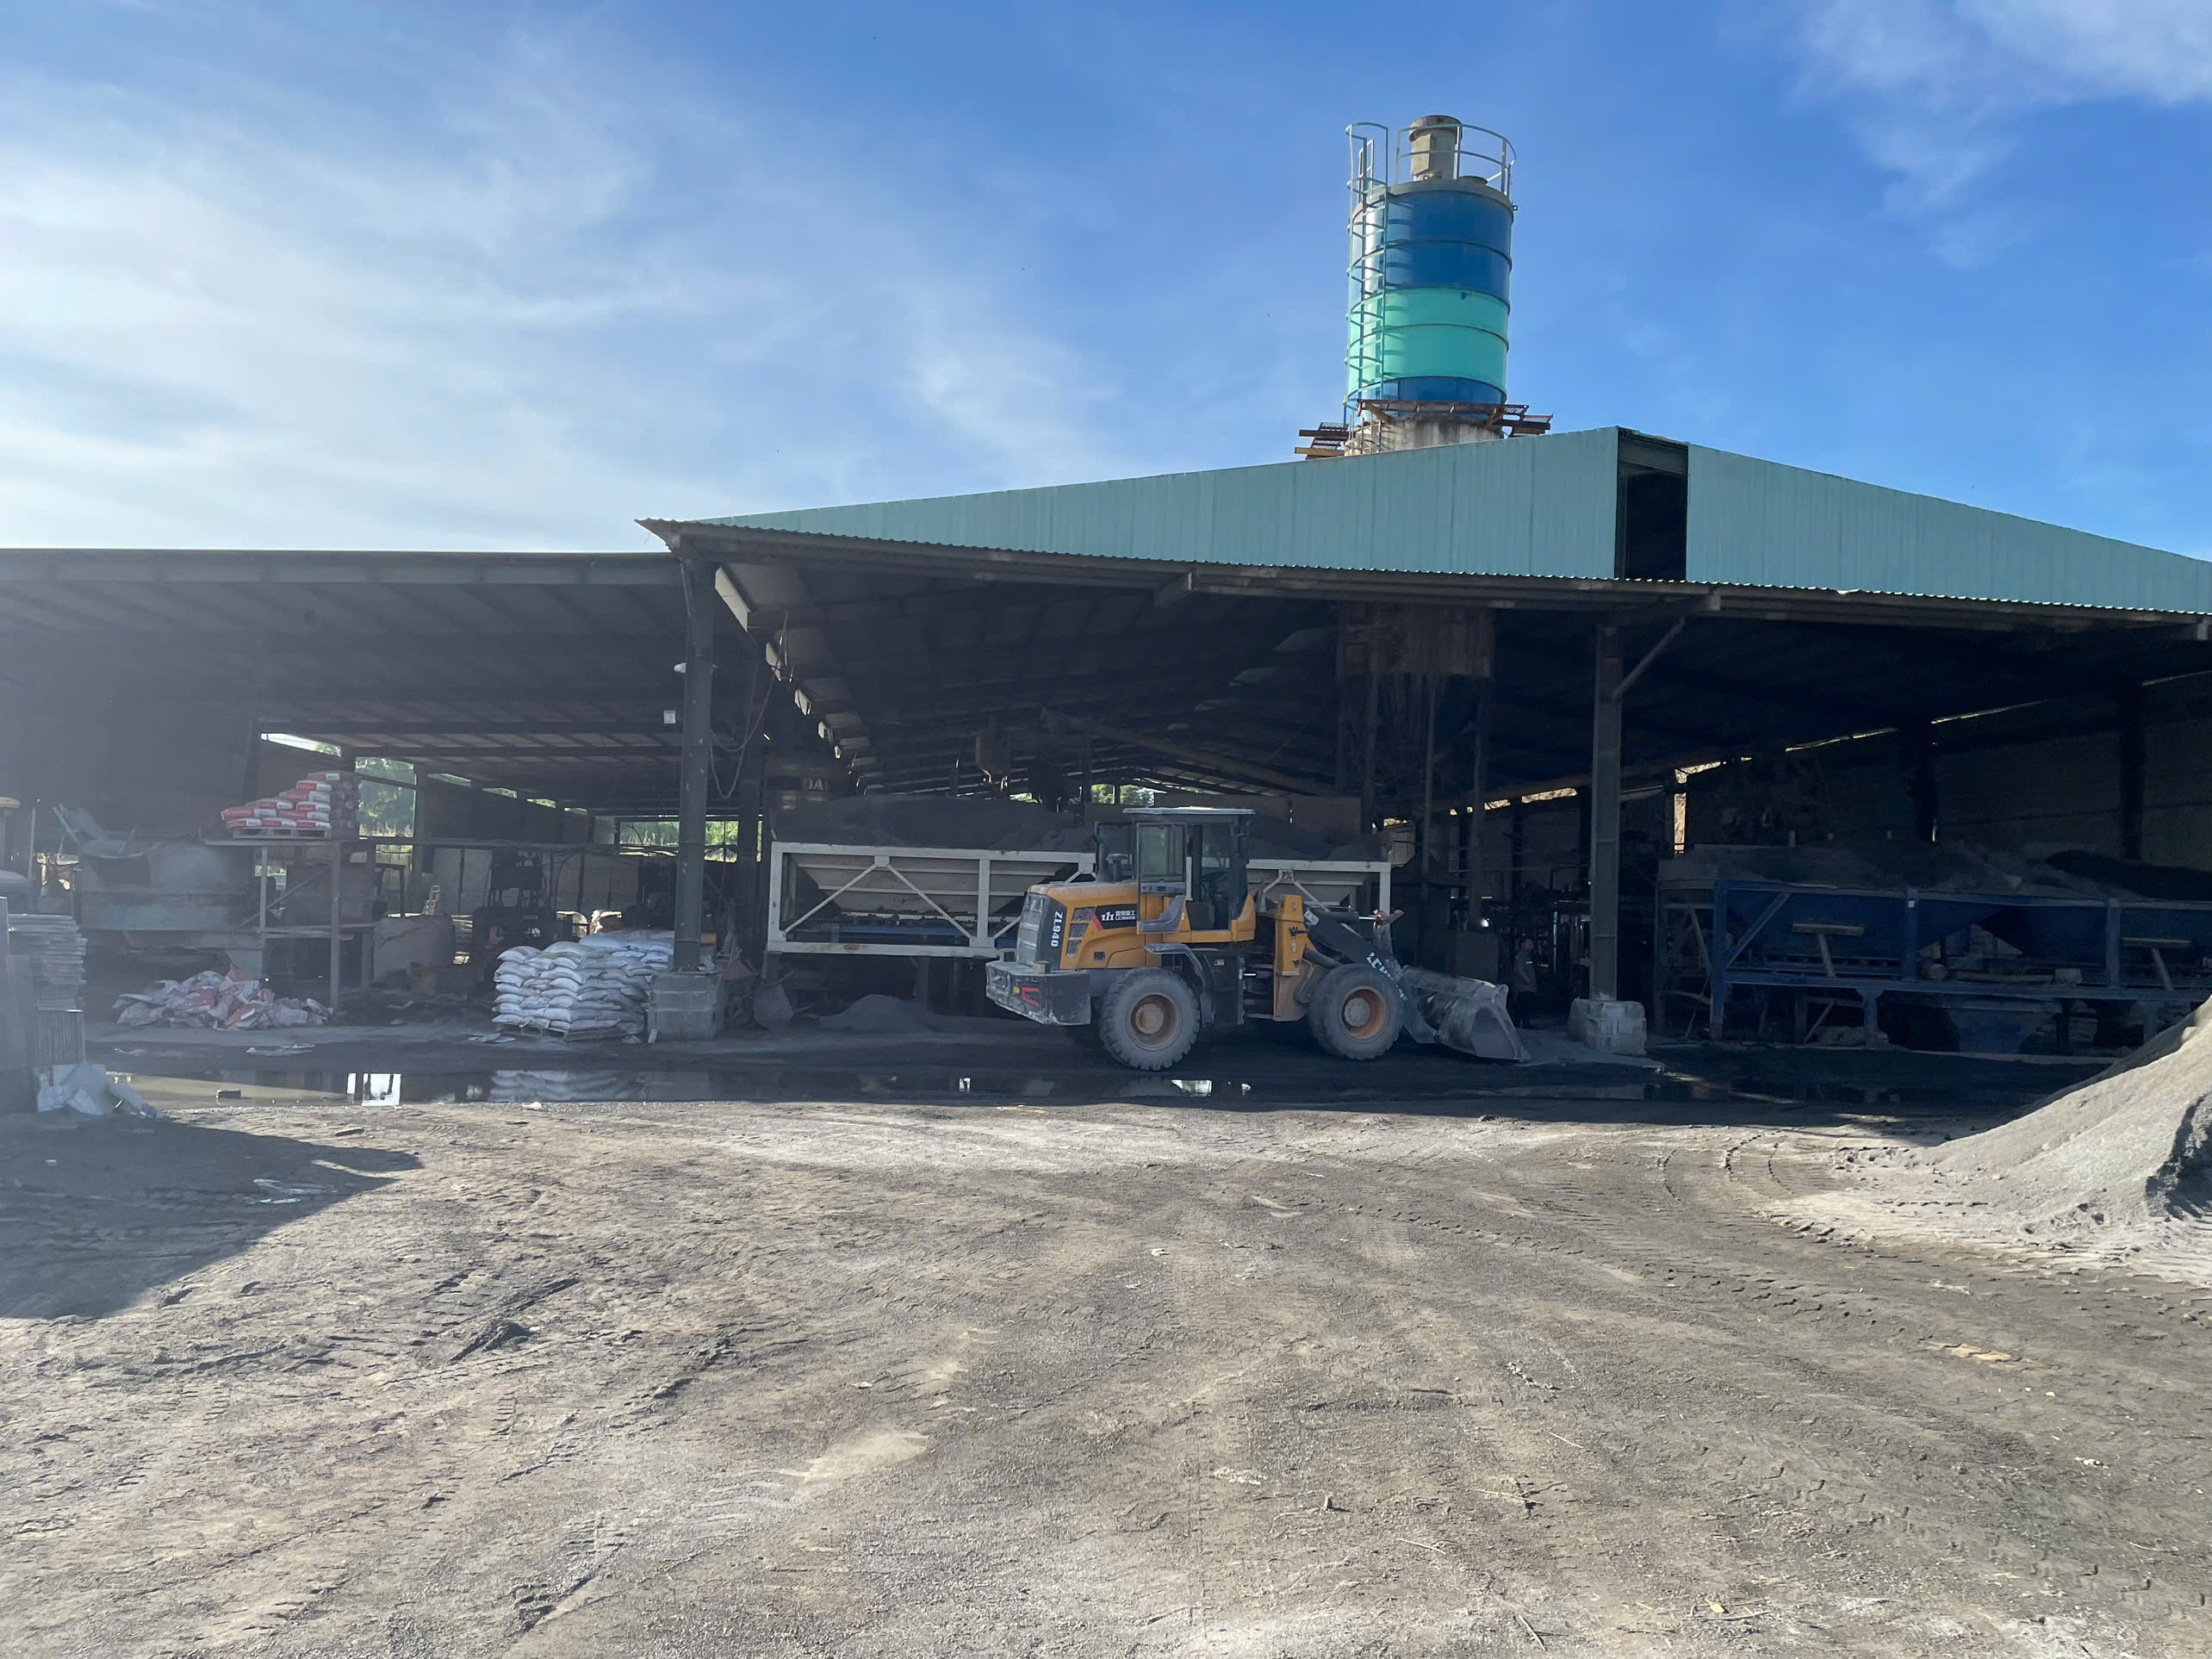
\includegraphics[width=\linewidth,height=3.8cm,keepaspectratio]{images/gia_quy_khu_xu_ly_da.jpg}
    \end{minipage}
    \caption{Selected examples from the Gia Quy visit: an olivine-bearing rock specimen (left), a white calcite specimen (centre), and the material-handling area (right).}
    \label{fig:resources_gia_quy_materials}
\end{figure}

The use of construction stone also has environmental costs. Quarrying and material handling can generate dust, noise, sediment-bearing runoff, and changes to land cover. Measures such as controlling dust at transfer points, maintaining haul roads, managing drainage, and progressively rehabilitating disturbed areas address these issues~\cite{quarry-ehs}. These measures provide a framework for discussing environmental management at the site.

Gia Quy and Ho Da together demonstrate why resource assessment should include both production and the later condition of the extraction site. Rock quality determines possible uses, excavation design affects access and stability, and environmental management influences the effects on surrounding land and water.

Granite at Mui Ke Ga provides another example from the coastal stops. The rocky shore allowed us to relate this geological material to weathering and marine erosion, processes described in our field notes~\cite{group-field-notes}. Together with andesite at Ho Da and basalt at Gia Quy, it illustrates the variety of rocks encountered during the survey. These examples are a selection from the materials studied, and their potential engineering uses still depend on material quality and appropriate evaluation.

\subsection{Petroleum Resources and Offshore Technology at Vietsovpetro}

Vietsovpetro was established on 19 June 1981 under an intergovernmental agreement between Vietnam and the Soviet Union. Its first crude oil was produced from Bach Ho field on 26 June 1986~\cite{vietsov-history}. These milestones provided historical context for the organization introduced during the visit. The development of petroleum resources involves establishing the technical capability to investigate the subsurface, construct wells, and support operations offshore; the exhibitions helped connect that wider activity with the models we could examine directly.

During our visit, the group viewed exhibition models and listened to explanations of the organization's activities. The offshore-field model showed multiple platforms, vessels, and connecting routes. Its main educational value was the arrangement of these components: a petroleum field depends on a coordinated system for drilling, production, material movement, and support.

The model helped us distinguish the resource beneath the seabed from the infrastructure needed to develop it. A platform is one part of that system, while other facilities and vessels contribute different functions. Following these relationships on the model helped us study the connection between Earth Science and industrial activity during the onshore exhibition visit.

\begin{figure}[H]
    \centering
    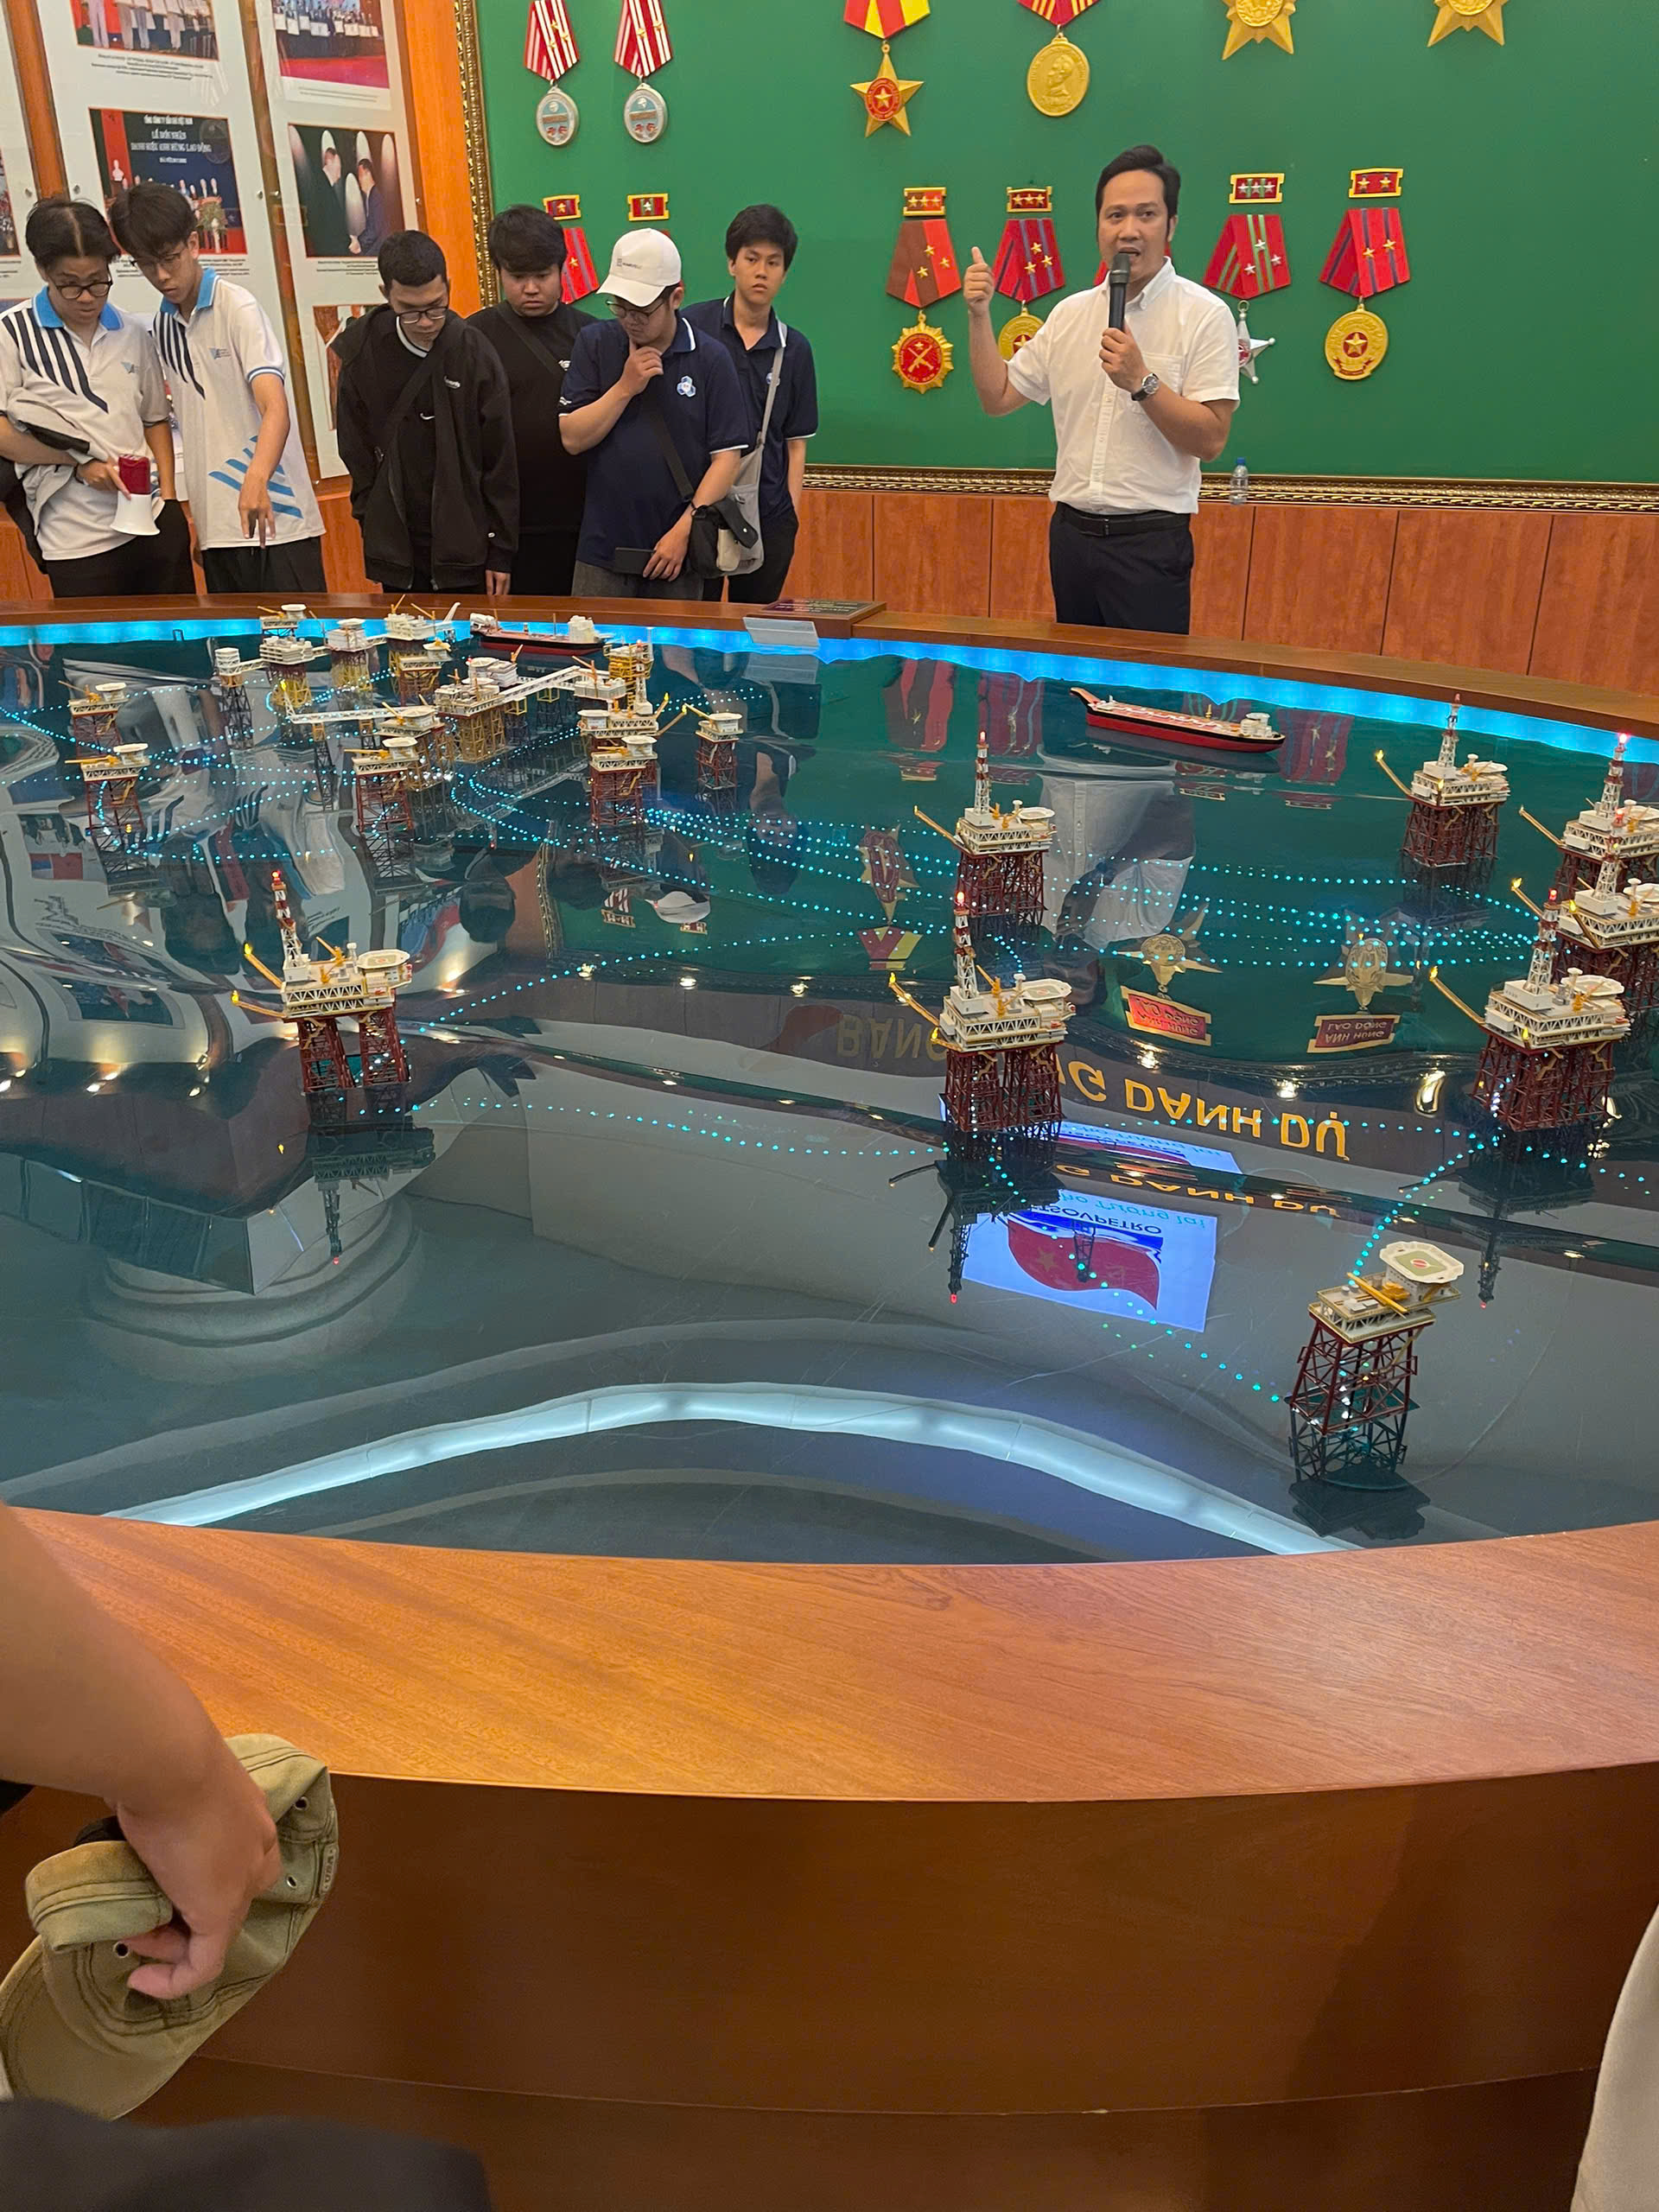
\includegraphics[height=8.5cm]{images/vietsovpetro_mo_hinh_mo_dau.jpg}
    \caption{The group listening to an explanation beside an offshore-field model at Vietsovpetro.}
    \label{fig:resources_vietsov_field_model}
\end{figure}

\subsubsection{Offshore Structures and Their Engineering Role}

The exhibits included a model labelled TAM DAO 02 and a platform model with a steel jacket supporting deck facilities. Vietsovpetro identifies Tam Dao 02 as a jack-up drilling rig~\cite{vietsov-facilities}. In the model, the drilling tower, working areas, and long supporting legs could be considered together. The adjacent platform model showed a different structural arrangement, with a braced steel framework beneath the deck. Comparing the exhibits helped us recognize that offshore development involves several types of structure with different roles.

The supporting legs also provide a connection to geotechnical engineering. A jack-up foundation must be assessed against the seabed geometry and the soil or rock conditions beneath the footing locations. Differences between those locations can affect the foundation response, so site surveys and subsurface investigations form part of the engineering assessment~\cite{offshore-foundations}. This relationship explains why understanding the ground remains important even when the main activity is taking place at sea.

The exhibition therefore illustrated two applications of Earth Science: knowledge used to develop a subsurface resource, and knowledge of seabed conditions used to support the structures that make development possible.

\begin{figure}[H]
    \centering
    \begin{minipage}[t]{0.47\textwidth}
        \centering
        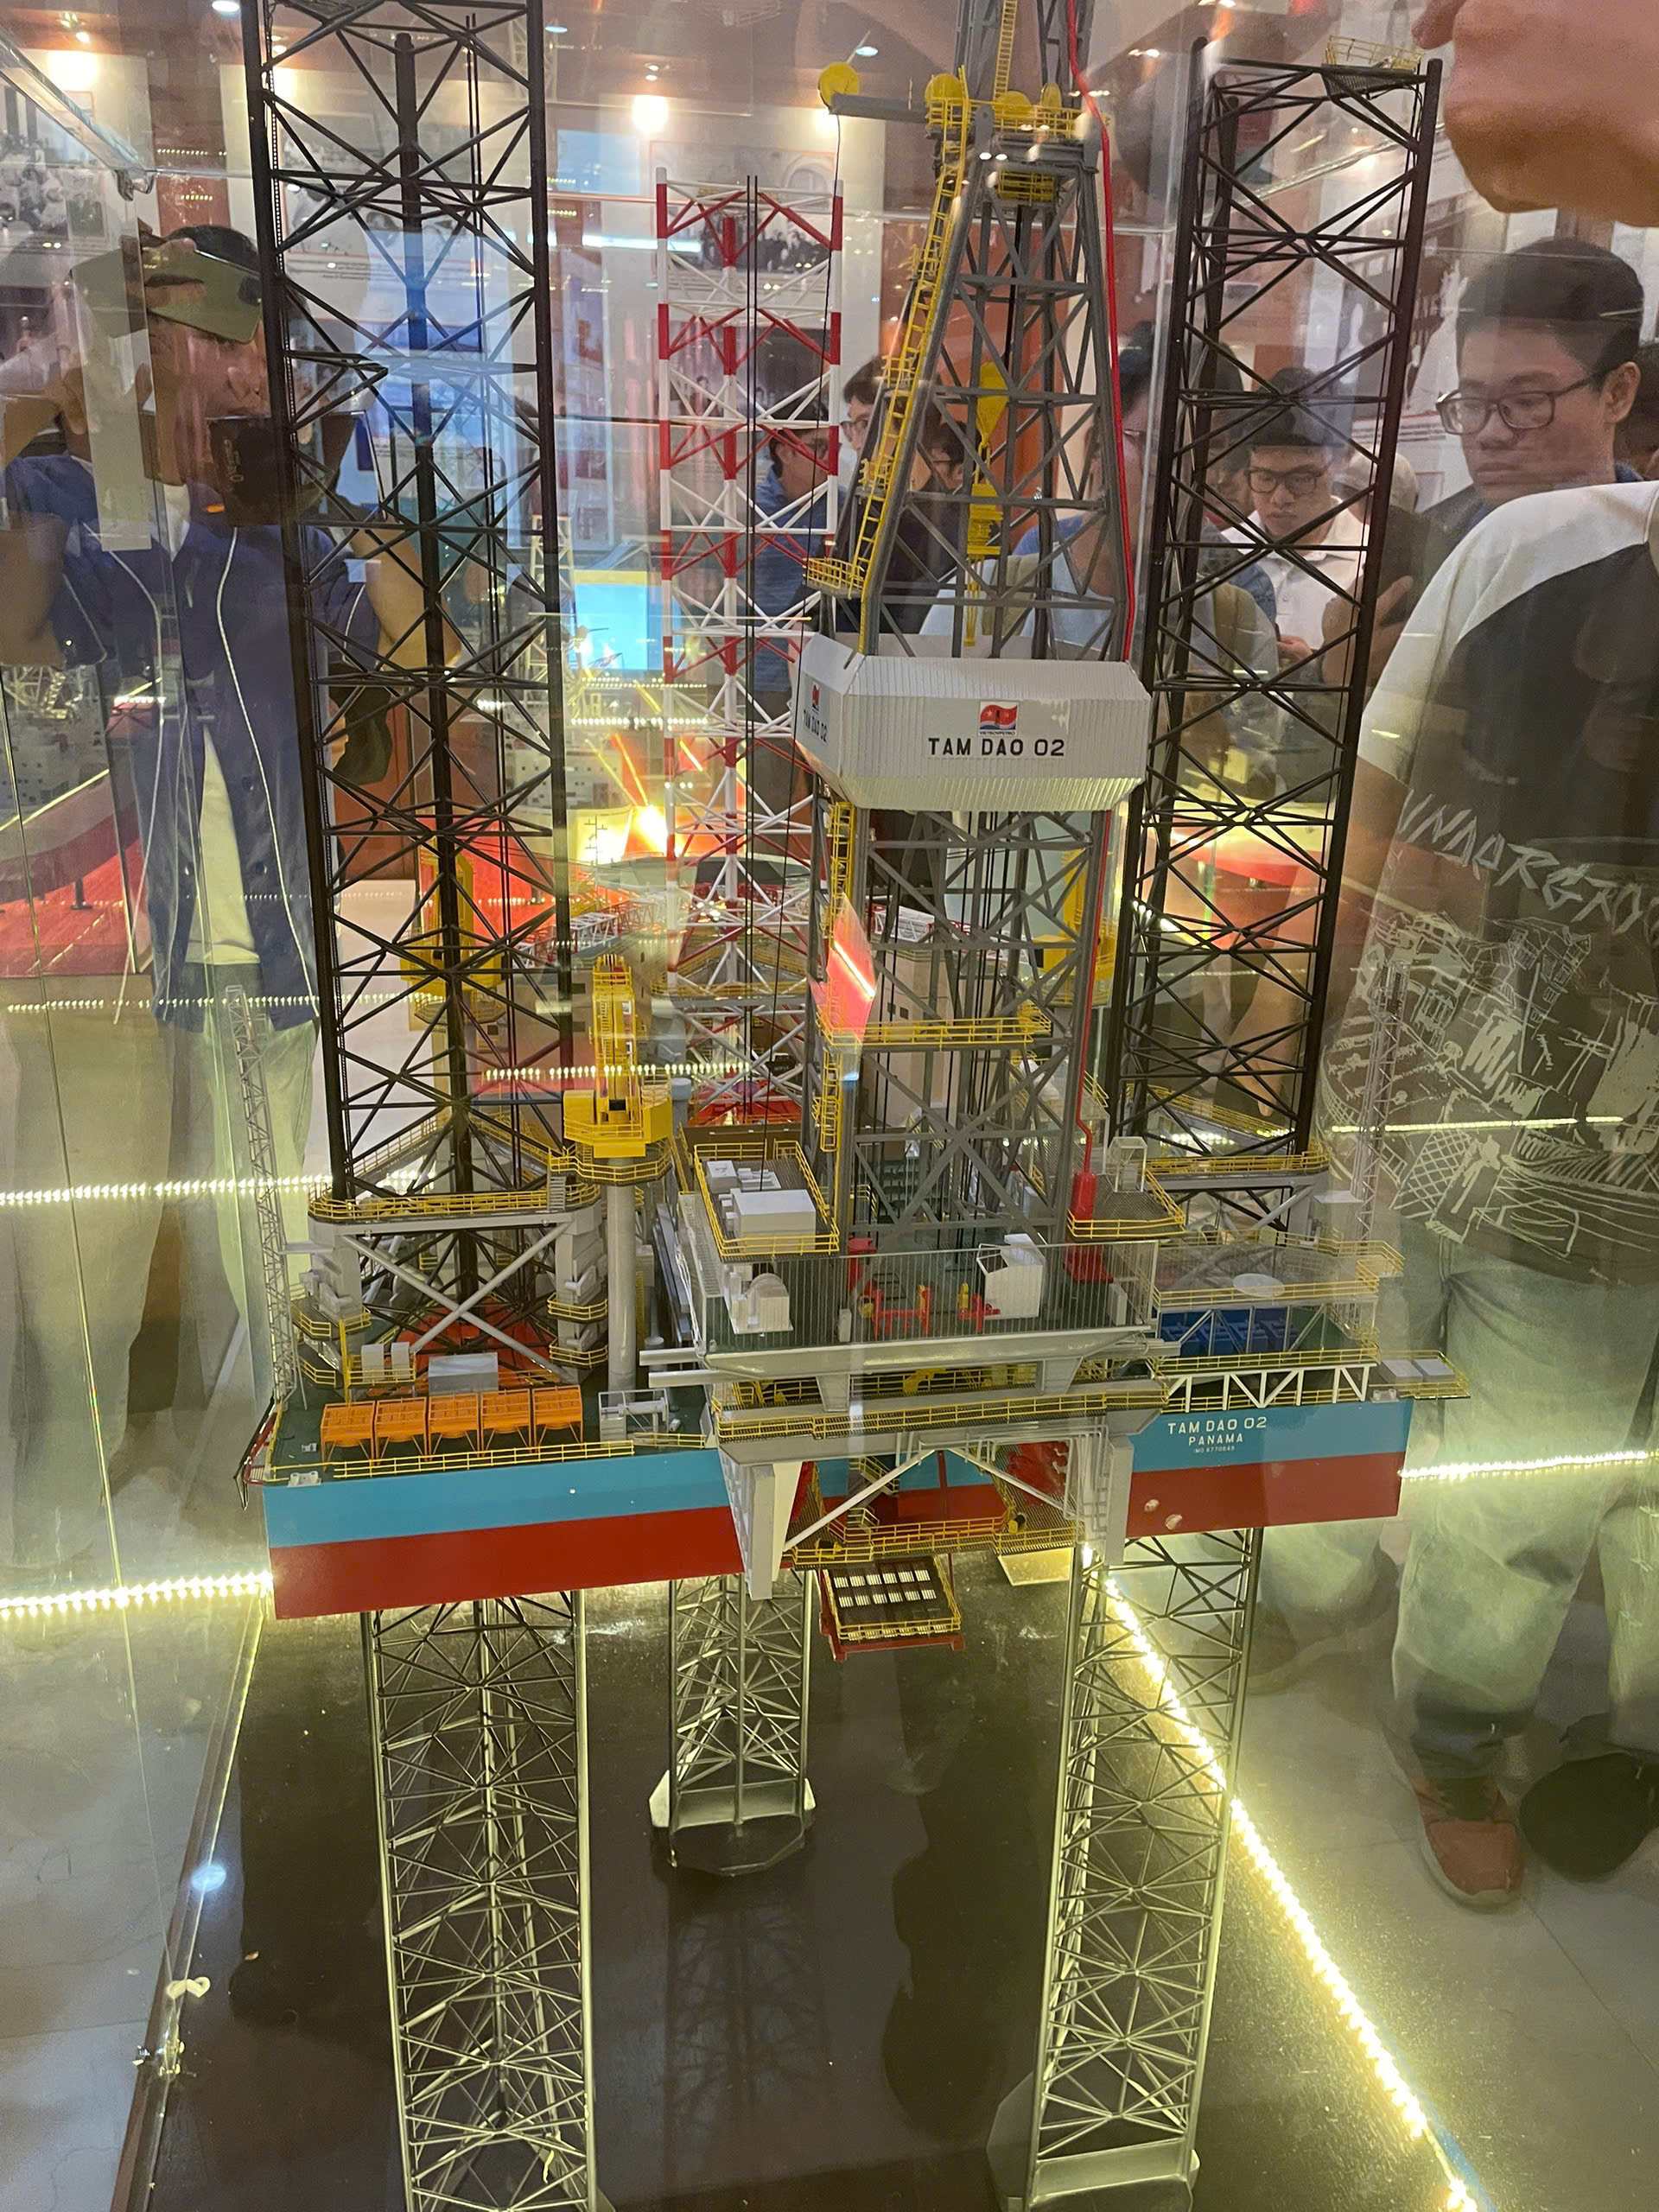
\includegraphics[height=7.1cm]{images/vietsovpetro_gian_khoan_tam_dao_02.jpg}
    \end{minipage}\hfill
    \begin{minipage}[t]{0.47\textwidth}
        \centering
        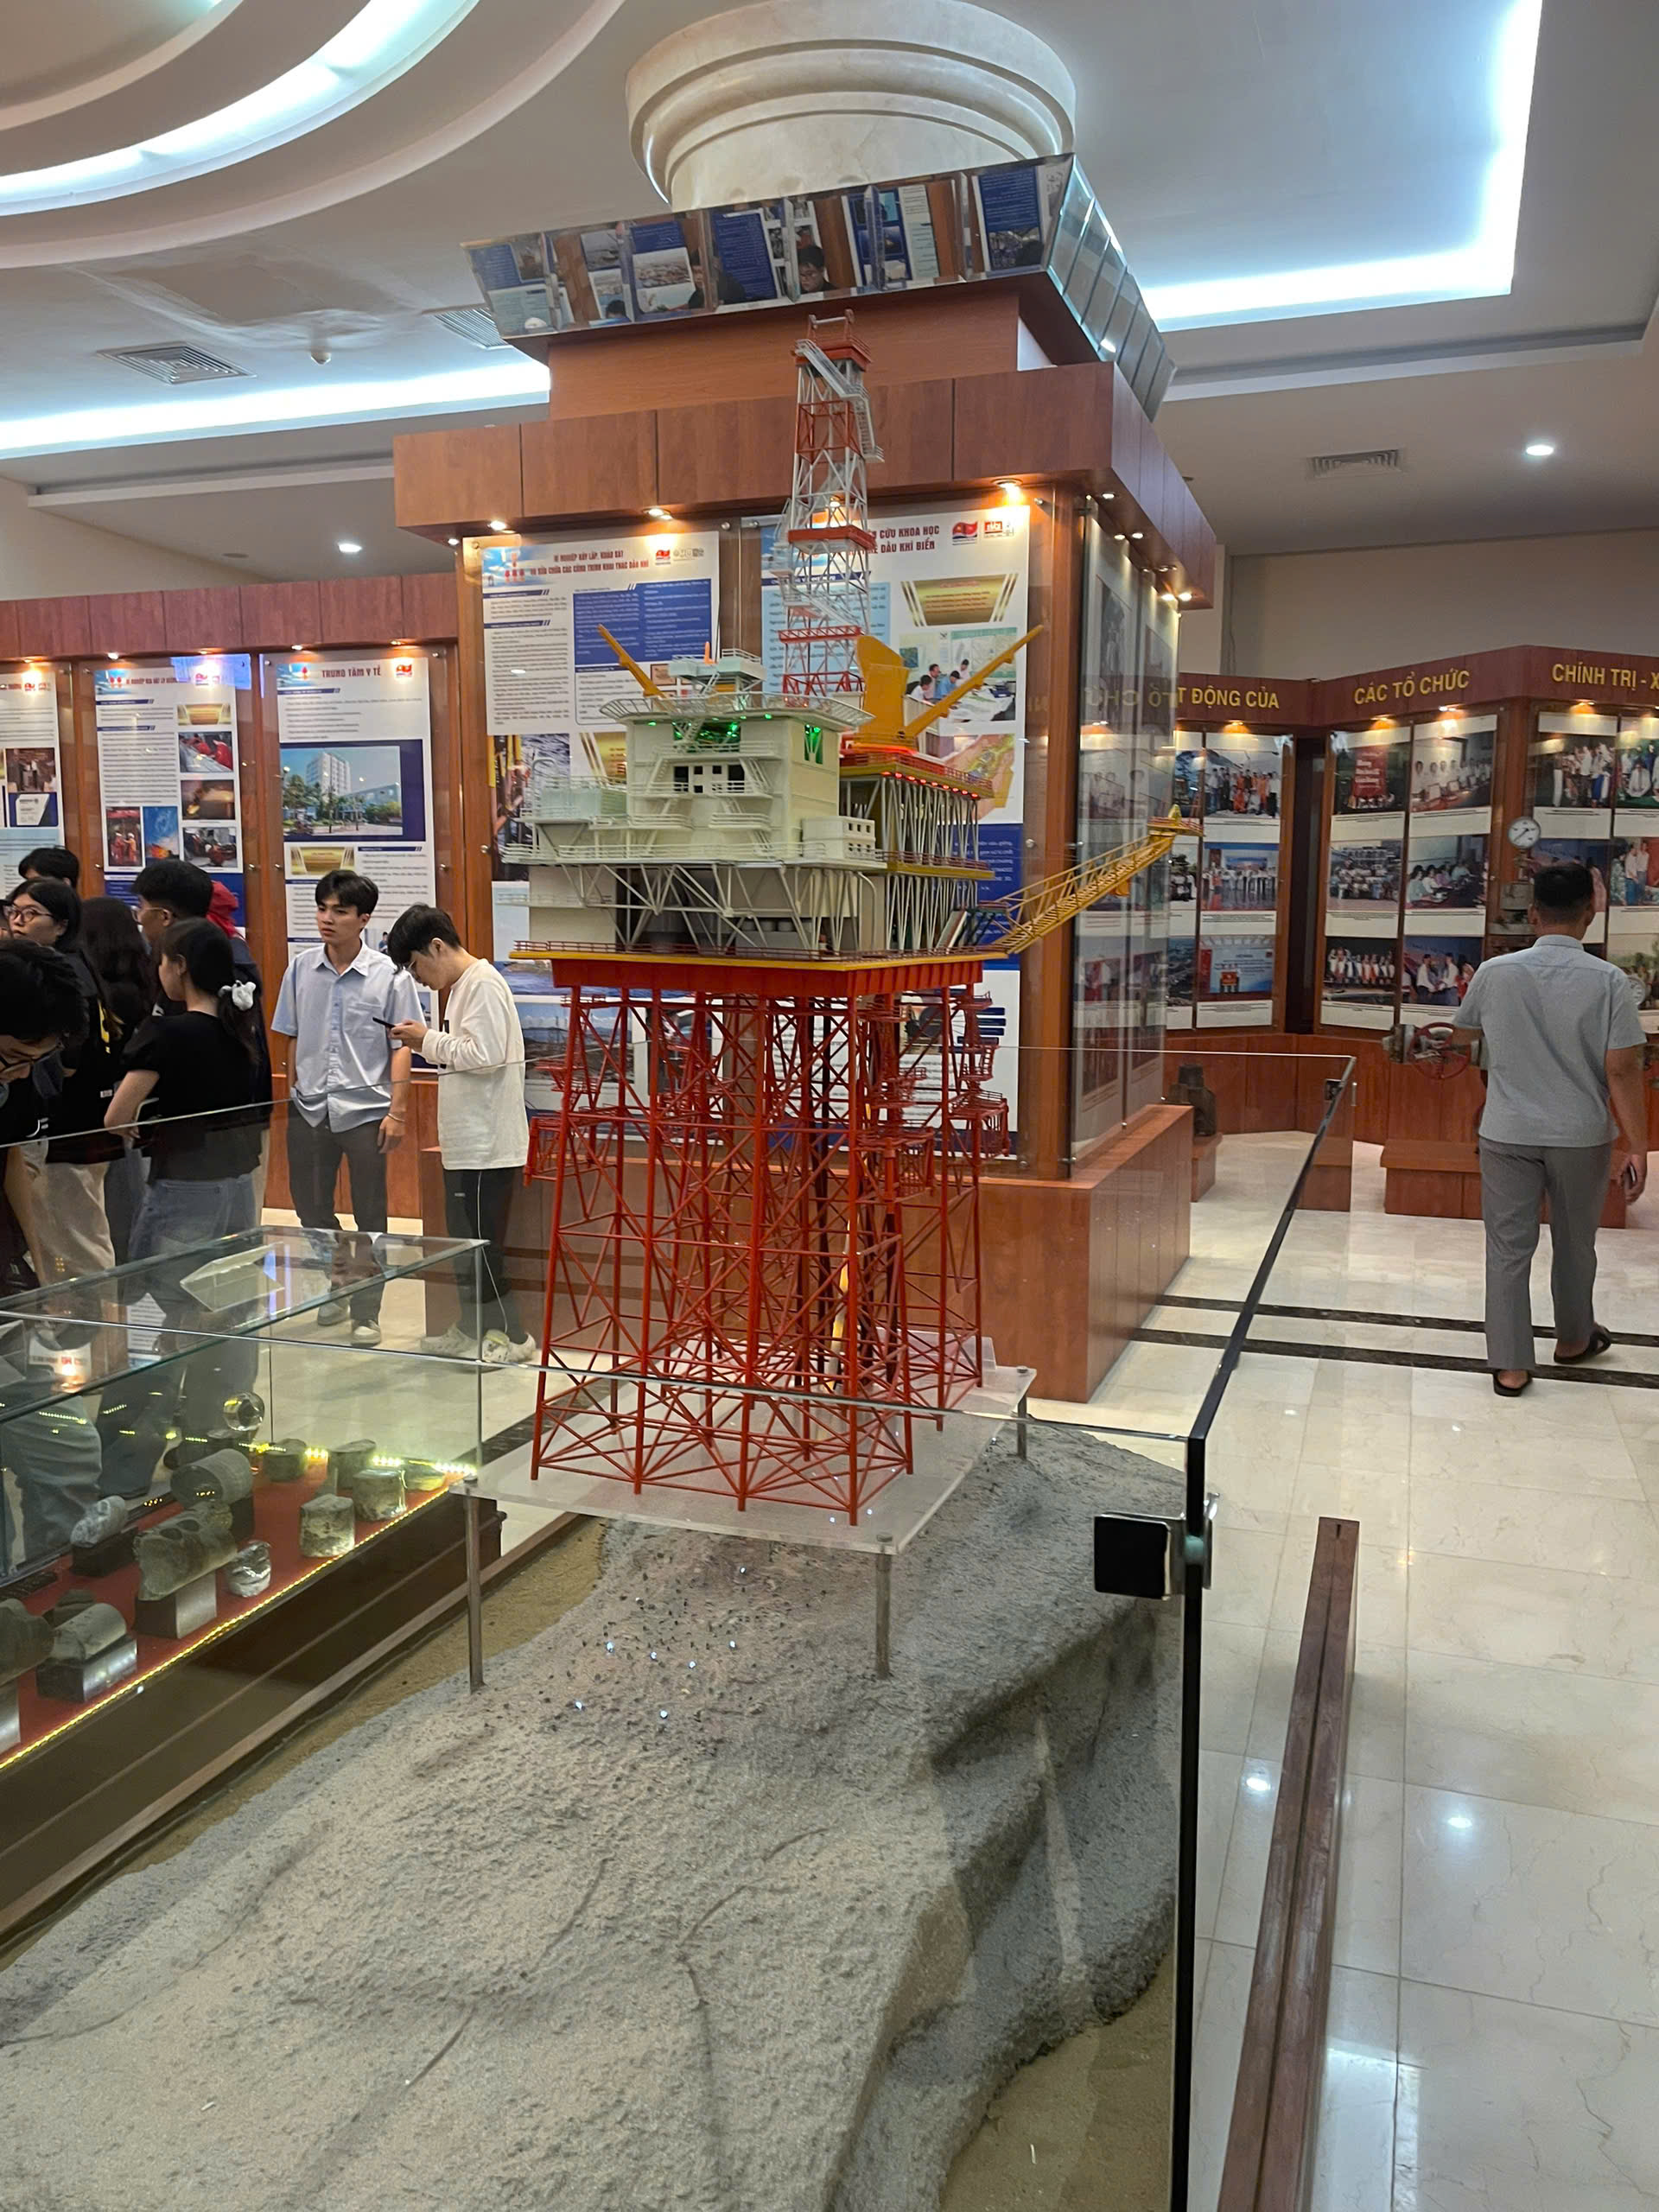
\includegraphics[height=7.1cm]{images/vietsovpetro_mo_hinh_gian_co_dinh.jpg}
    \end{minipage}
    \caption{Exhibition models of TAM DAO 02 (left) and an offshore platform with a steel jacket and deck facilities (right).}
    \label{fig:resources_vietsov_platforms}
\end{figure}

\subsubsection{Drilling Technology and Economic Efficiency}

One point introduced during the visit concerned the economic benefit of wear-resistant diamond cutting elements. This gave us an example of how a change in material technology can influence the cost of accessing a geological resource. The relevant tool is the drill bit, located at the bottom of the drillstring, where it cuts or breaks the formation.

Polycrystalline diamond compact (PDC) bits use synthetic diamond cutting elements mounted on a supporting body. That body may itself be steel or a tungsten-carbide matrix. The diamond is used at the cutting surface, where resistance to wear is important. PDC cutters remove rock by a shearing action, while roller-cone bits use rolling cutting structures to break the formation~\cite{drill-bit-technology}. The tools illustrate how cutting materials and bit design affect rock removal.

A study by Vietsovpetro researchers reports that PDC bits were first used at the company's wells in 1994. It describes continued improvements to cutter materials, bit geometry, and compatibility with drilling systems for the Tertiary sedimentary formations of Bach Ho and Rong fields~\cite{vietsov-pdc}. This provides technical support for the improvement in drilling efficiency discussed during the visit.

The economic reasoning is straightforward. When a bit maintains useful cutting performance for a longer interval, more metres can be drilled before replacement becomes necessary. Changing a worn bit involves withdrawing the drillstring and returning the replacement assembly to the bottom of the well. Reducing such interruptions can save operating time. Improved drilling speed and longer useful intervals can therefore contribute to a lower overall well-construction cost~\cite{drill-bit-technology,vietsov-pdc}.

The economic comparison must include the complete drilling operation: the bit, equipment time, drilling progress, and replacement work. A wear-resistant cutter is useful when its performance suits the rock and operating conditions. The Vietsovpetro study similarly emphasizes selecting and improving bits for particular well structures and geological conditions~\cite{vietsov-pdc}. The explanation we received highlights potential savings in total drilling cost through improved tool performance.

Across the three resource-related stops, the main connection was between geology and decisions about use. At a quarry, those decisions concern material selection, excavation, and the future landscape. At an offshore petroleum operation, they also concern the design of structures and the performance of drilling tools. The fieldtrip helped us see how technical knowledge affects both the economic value obtained from a resource and the responsibilities associated with its development.

\section{Conclusion}
This field trip was a truly unforgettable experience for all members of our group. It was not only a journey to observe rocks, landforms, coastal environments, and natural resources, but also a meaningful opportunity for us to connect classroom knowledge with real field observations. Through each stop of the trip, we learned how Earth Science concepts appear in the real world, from weathering, erosion, and igneous rocks to groundwater, coastal processes, mangrove forests, atmospheric hazards, and natural resource exploitation.

During the fieldtrip, our group had the opportunity to learn about different types of rocks, including intrusive igneous rocks and extrusive volcanic rocks. We observed how magma-related processes can form rocks such as granite, diabase, basalt, and rhyolite, and how these rocks are later modified by weathering, erosion, and human activities. These observations helped us understand geological processes more clearly than learning from textbooks alone.

The fieldtrip also allowed us to apply practical field skills in real situations. We used knowledge of field observation, sample collection, note-taking, photography, and geological description directly at outcrops. In particular, we had the chance to apply compass-related knowledge in the field, which helped us understand how basic field equipment can support geological observation and measurement. These experiences made Earth Science more realistic, practical, and memorable for us.

Every group member had the chance to participate in field activities such as observing outcrops, collecting samples, taking photographs, recording notes, and discussing geological features. These activities helped us realize that Earth Science is not only about theories in lectures, but also about careful observation, teamwork, patience, and curiosity in the field. The trip also allowed us to become closer as a group, as we worked together, supported one another, and shared many memorable moments throughout the journey.

We would like to express our deepest gratitude to Dr. Nguyen Thu Thuy for her dedication, enthusiasm, and tireless teaching throughout the fieldtrip. Despite the long travel schedule and challenging outdoor conditions, she continuously explained the geological features at each site with great energy and passion. Her guidance helped us better understand the meaning of each observation and inspired us to appreciate Earth Science more deeply.

We would also like to sincerely thank MSc. Le Thanh Phong and all the lecturers who organized this fieldtrip. Their careful preparation, guidance, and support created a valuable learning environment for students. Thanks to their efforts, we were able to visit important geological, coastal, and industrial sites and gain practical knowledge that would be difficult to obtain in a classroom setting alone.

In addition, our group would like to thank the supporting staff members and especially Mr. Ngo Tan Tien for assisting our group and the whole fieldtrip team during the journey. Their support helped the trip run smoothly and safely, allowing students to focus on learning, observing, and completing field tasks.

Overall, this fieldtrip will remain a precious and unforgettable memory for all members of our group. It gave us not only academic knowledge, but also practical field experience, friendship, teamwork, gratitude, and respect for nature. We believe that this fieldtrip was more than an academic activity; it was a journey of learning, appreciation, and memories that will stay with us for a long time.

\clearpage
\begin{thebibliography}{99}

\bibitem{1} Vietnam Disaster Management Authority. Vietnam floods response plan 31 october 2020. \url{https://phongchongthientai.mard.gov.vn/en/Pages/vietnam-floods-response-plan--31-october-2020.aspx}, 2020. Accessed May 2026.

\bibitem{2} VinWonders. Typhoon season in vietnam: Timing, risks, and travel advice. \url{https://vinwonders.com/en/wonderpedia/news/vietnam-typhoon-season/}, 2025. Accessed May 2026.

\bibitem{3} Wikipedia contributors. Climate of vietnam. \url{https://en.wikipedia.org/wiki/Climate_of_Vietnam}, 2026. Accessed May 2026.

\bibitem{4} Wikipedia contributors. Tropical cyclones in vietnam. \url{https://en.wikipedia.org/wiki/Tropical_cyclones_in_Vietnam}, 2026. Accessed May 2026.


\bibitem{climate-qcvn} Ministry of Construction. \textit{QCVN 02:2022/BXD: National Technical Regulation on Natural Physical and Climatic Data for Construction}. Tables A.2, A.10, and A.25, 2022. \url{https://datafiles.chinhphu.vn/cpp/files/vbpq/2022/10/02-bxd.pdf}.

\bibitem{climate-phanthiet} People's Committee of Phan Thiet City. \textit{Explanatory Report on the 2023 Land-Use Plan of Phan Thiet City}. Section 1.1.3: Climate, p.\ 8, 2023. \url{https://storage-vnportal.vnpt.vn/btn-ubnd/4776/CongkhaiKHSDD2023/BAO%20CAO%20KHSDD%202023%20PHAN%20THIET%20NGAY%2012062023.pdf}.

\bibitem{wind-transport} National Park Service. \textit{Monitoring Aeolian Features and Processes}. \url{https://www.nps.gov/articles/aeolian.htm}.


\bibitem{group-field-notes} Fieldtrip group. \textit{Field notebook (Nhat ky)}. Entries for Ho Da, Gia Quy, and Mui Ke Ga, 30--31 October 2026. Unpublished field notes supplied with this report.

\bibitem{aggregate-geology} W. H. Langer and D. H. Knepper, Jr. \textit{Geologic Characterization of Natural Aggregate}. U.S. Geological Survey Open-File Report 95-582, 1995. \url{https://pubs.usgs.gov/of/1995/ofr-95-0582/ofr-95-0582.pdf}.

\bibitem{aggregate-uses} T. I. Nelson and W. P. Bolen. \textit{Construction Aggregates}. U.S. Geological Survey, 2007. \url{https://www.usgs.gov/publications/construction-aggregates}.

\bibitem{quarry-ehs} International Finance Corporation. \textit{Environmental, Health, and Safety Guidelines for Construction Materials Extraction}. 2007. \url{https://www.ifc.org/content/dam/ifc/doc/2000/2007-construction-materials-extraction-ehs-guidelines-en.pdf}.

\bibitem{vietsov-history} Vietsovpetro. \textit{History of Formation}. \url{https://www.vietsov.com.vn/_catalogs/masterpage/lichsu.aspx}.

\bibitem{vietsov-facilities} Vietsovpetro. \textit{Facilities and Equipment}. \url{https://www.vietsov.com.vn/_catalogs/masterpage/cosovatchat.aspx}.

\bibitem{drill-bit-technology} SLB. \textit{The Defining Series: Bits}. 2016. \url{https://www.slb.com/resource-library/oilfield-review/defining-series/defining-bits}.

\bibitem{vietsov-pdc} Đặng Của, Bùi Lê Trọng Hóa, Tạ Ngọc Ánh, Tạ Văn Thịnh, and Nguyễn Văn Cường. \textit{Improving the Structure of Polycrystalline Diamond Compact Drill Bit to Enhance Efficiency When Drilling Through Tertiary Sediments of Bach Ho and Rong Fields, Cuu Long Basin}. Petrovietnam Journal, no.\ 3, pp.\ 57--65, 2024. \url{https://doi.org/10.47800/PVSI.2024.03-06}.


\bibitem{field-minerals} National Park Service. \textit{Minerals}. Sections on olivine and calcite. \url{https://www.nps.gov/subjects/geology/minerals.htm}.

\bibitem{quarry-highwalls} C. Haycocks, G. Haycocks, and Y. Zhou. \textit{Long-term Stability of Abandoned Quarry Highwalls}. 1991. NIOSH Mining Publications. \url{https://stacks.cdc.gov/view/cdc/245526}.

\bibitem{offshore-foundations} L. Kellezi, G. Kudsk, and H. Hofstede. \textit{Jack-up Rig Foundation Design Applying 3D FE Structure--Soil--Interaction Modelling}. Proceedings of the BGA International Conference on Foundations, Dundee, 2008. \url{https://www.geo.dk/media/1184/538_1275_kell_dk_kuds_dk_hofs_nl_070208_rmm.pdf}.

\end{thebibliography}

\end{document}
```eof
